\documentclass{ximera}

%% You can put user macros here
%% However, you cannot make new environments

\listfiles

\graphicspath{{./}{firstExample/}{secondExample/}}

\usepackage{tikz}
\usepackage{tkz-euclide}
\usepackage{tikz-3dplot}
\usepackage{tikz-cd}
\usetikzlibrary{shapes.geometric}
\usetikzlibrary{arrows}
\usetikzlibrary{decorations.pathmorphing,patterns}
\usetkzobj{all}
\pgfplotsset{compat=1.13} % prevents compile error.

\renewcommand{\vec}[1]{\mathbf{#1}}
\newcommand{\RR}{\mathbb{R}}
\newcommand{\dfn}{\textit}
\newcommand{\dotp}{\cdot}
\newcommand{\id}{\text{id}}
\newcommand\norm[1]{\left\lVert#1\right\rVert}
 
\newtheorem{general}{Generalization}
\newtheorem{initprob}{Exploration Problem}

\tikzstyle geometryDiagrams=[ultra thick,color=blue!50!black]

\usepackage{mathtools}

\title{Constant Coefficient Homogeneous Systems II}%\label{Module 7-ADEF}


\begin{document}

\begin{abstract}

\end{abstract}

\maketitle

\section*{Constant Coefficient Homogeneous Systems II}

We saw in \href{https://ximera.osu.edu/ode/main/constCoeffHomSysI/constCoeffHomSysI}{Trench 10.4} that if an $n\times n$
constant matrix
$A$ has $n$ real eigenvalues $\lambda_1, \lambda_2, \dots, \lambda_n$
(which need not be distinct) with associated linearly independent
eigenvectors ${\bf x}_1, {\bf x}_2, \dots, {\bf x}_n$, then the general
solution of ${\bf y}'=A{\bf y}$ is
$$
{\bf y}=c_1{\bf x}_1e^{\lambda_1t}+c_2{\bf x}_2e^{\lambda_2 t}
+\cdots+c_n{\bf x}_ne^{\lambda_n t}.
$$
In this section we consider the case where $A$ has $n$ real
eigenvalues, but does not have $n$ linearly independent eigenvectors.
It is shown in linear algebra that this occurs if and only if $A$ has
at least one eigenvalue of multiplicity $r>1$ such that the associated
eigenspace has dimension less than $r$. In this case $A$ is said to be
\dfn{defective}. Since it's beyond the scope of this book to give a
complete analysis of systems with defective coefficient matrices, we
will restrict our attention to some commonly occurring special cases.

\begin{example}\label{example:10.5.1}
Show that the system
\begin{equation}\label{eq:10.5.1}
{\bf y}'=\begin{bmatrix}11&-25\\4&-9\end{bmatrix}{\bf y}
\end{equation}
does not have a fundamental set of solutions of the form $\{{\bf
x}_1e^{\lambda_1t},{\bf x}_2e^{\lambda_2t}\}$, where $\lambda_1$ and
$\lambda_2$ are eigenvalues of the coefficient matrix $A$ of
\eqref{eq:10.5.1} and ${\bf x}_1$, and ${\bf x}_2$ are associated
linearly independent eigenvectors.

\begin{explanation}   
The characteristic polynomial of $A$ is
\begin{eqnarray*}
\begin{vmatrix}11-\lambda&-25\\4&-9-\lambda\end{vmatrix}
&=&(\lambda-11)(\lambda+9)+100\\
&=&\lambda^2-2\lambda+1=(\lambda-1)^2.
\end{eqnarray*}
Hence, $\lambda=1$ is the only eigenvalue of $A$. The augmented
matrix of the system $(A-I){\bf x}={\bf 0}$ is
$$
\begin{bmatrix}10&-25&\vdots&0\\4&
-10&\vdots&0\end{bmatrix},
$$
which is row equivalent to
$$
\begin{bmatrix}1&-5/2&\vdots&0\\0&
0&\vdots&0\end{bmatrix}.
$$
Hence, $x_1=\frac{5}{2}x_2$ where $x_2$ is arbitrary. Therefore all
eigenvectors of $A$ are scalar multiples of ${\bf
x}_1=\begin{bmatrix}5\\2\end{bmatrix}$,
so $A$ does not have a set of two linearly independent eigenvectors.
\end{explanation}
\end{example}

From Example~\ref{example:10.5.1}, we know that all scalar multiples of
${\bf y}_1=\begin{bmatrix}5\\2\end{bmatrix}e^t$ are solutions of \eqref{eq:10.5.1};
however,
to find the general solution we must find a second solution ${\bf
y}_2$ such that $\{{\bf y}_1,{\bf y}_2\}$ is linearly independent.
Based on your recollection of the procedure for solving a constant
coefficient scalar equation
$$
ay''+by'+cy=0
$$
in the case where the characteristic polynomial has a repeated root,
you might expect to obtain a second solution of \eqref{eq:10.5.1} by
multiplying the first solution by $t$. However, this yields ${\bf
y}_2=\begin{bmatrix}5\\2\end{bmatrix}te^t$, which doesn't work, since
$$
{\bf y}_2'=\begin{bmatrix}5\\2\end{bmatrix}(te^t+e^t),\quad\mbox{while}\quad
\begin{bmatrix}11&-25\\4&-9\end{bmatrix}{\bf y}_2=\begin{bmatrix}5\\2\end{bmatrix}te^t.
$$

The next theorem shows what to do in this situation.

\begin{theorem}\label{thmtype:10.5.1}
Suppose the $n\times n$ matrix $A$ has an eigenvalue $\lambda_1$
of multiplicity $\geq 2$ and the associated eigenspace has dimension
$1$ that is, all $\lambda_1$-eigenvectors of $A$ are scalar
multiples
of  an eigenvector ${\bf x}$.  Then there are infinitely many vectors
${\bf u}$ such that
\begin{equation}\label{eq:10.5.2}
(A-\lambda_1I){\bf u}={\bf x}.
\end{equation}
Moreover, if ${\bf u}$ is any such vector  then
\begin{equation}\label{eq:10.5.3}
{\bf y}_1={\bf x}e^{\lambda_1t}\quad\mbox{and}\quad
{\bf y}_2={\bf u}e^{\lambda_1t}+{\bf x}te^{\lambda_1t}
\end{equation}
are linearly independent  solutions of ${\bf y}'=A{\bf y}.$
\end{theorem}

A complete proof of this theorem is beyond the scope of this book. The
difficulty is in proving that there's a vector ${\bf u}$ satisfying
\eqref{eq:10.5.2}, since $\det(A-\lambda_1I)=0$. We'll take this without
proof and verify the other assertions of the theorem.

We already know that ${\bf y}_1$ in \eqref{eq:10.5.3} is a solution of
${\bf y}'=A{\bf y}$. To see that ${\bf y}_2$ is also a solution, we
compute
\begin{eqnarray*}
{\bf y}_2'-A{\bf y}_2&=&\lambda_1{\bf u}e^{\lambda_1t}+{\bf
x} e^{\lambda_1t}
+\lambda_1{\bf x} te^{\lambda_1t}-A{\bf
u}e^{\lambda_1t}-A{\bf x} te^{\lambda_1t}\\
&=&(\lambda_1{\bf u}+{\bf x} -A{\bf
u})e^{\lambda_1t}+(\lambda_1{\bf x} -A{\bf x} )te^{\lambda_1t}.
\end{eqnarray*}
Since $A{\bf x}=\lambda_1{\bf x}$, this can be written as
$$
{\bf y}_2'-A{\bf y}_2=-
\left((A-\lambda_1I){\bf u}-{\bf x}\right)e^{\lambda_1t},
$$
and now \eqref{eq:10.5.2} implies that
${\bf y}_2'=A{\bf y}_2$.

To see that ${\bf y}_1$ and ${\bf y}_2$  are linearly independent,
suppose   $c_1$ and $c_2$ are constants such that
\begin{equation}\label{eq:10.5.4}
c_1{\bf y}_1+c_2{\bf y}_2=c_1{\bf x}e^{\lambda_1t}+c_2({\bf
u}e^{\lambda_1t} +{\bf x}te^{\lambda_1t})={\bf 0}.
\end{equation}
We must show that $c_1=c_2=0$.  Multiplying \eqref{eq:10.5.4}
by $e^{-\lambda_1t}$ shows that
\begin{equation}\label{eq:10.5.5}
c_1{\bf x}+c_2({\bf u} +{\bf x}t)={\bf 0}.
\end{equation}
By differentiating this with respect to $t$, we see that $c_2{\bf
x}={\bf 0}$, which implies $c_2=0$, because ${\bf x}\neq{\bf 0}$.
Substituting  $c_2=0$ into \eqref{eq:10.5.5}  yields $c_1{\bf x}={\bf 0}$,
which implies that $c_1=0$, again because ${\bf x}\neq{\bf 0}$

\begin{example}\label{example:10.5.2}
Use Theorem~\ref{thmtype:10.5.1} to find the general solution of the system
\begin{equation}\label{eq:10.5.6}
{\bf y}'=\begin{bmatrix}11&-25\\4&-9\end{bmatrix}{\bf y}
\end{equation}
considered in Example~\ref{example:10.5.1}.

\begin{explanation} 
In Example~\ref{example:10.5.1} we saw that $\lambda_1=1$ is an
eigenvalue of multiplicity $2$ of the coefficient matrix $A$ in
\eqref{eq:10.5.6}, and that all of the eigenvectors of $A$ are multiples of
$$
{\bf x}=\begin{bmatrix}5\\2\end{bmatrix}.
$$
Therefore
$$
{\bf y}_1=\begin{bmatrix}5\\2\end{bmatrix}e^t
$$
is a solution of \eqref{eq:10.5.6}. From Theorem~\ref{thmtype:10.5.1}, a second
solution is given by ${\bf y}_2={\bf u}e^t+{\bf x}te^t$, where
$(A-I){\bf u}={\bf x}$. The augmented matrix of this system is
$$
\begin{bmatrix}10&-25&\vdots&5\\4&-10&\vdots&2\end{bmatrix},
$$
which is row equivalent to
$$
\begin{bmatrix}1&-5/2&\vdots&1/2\\
0&0&\vdots&0\end{bmatrix}.
$$
Therefore the components of ${\bf u}$ must satisfy
$$
u_1-\frac{5}{2}u_2=\frac{1}{2},
$$
where  $u_2$ is arbitrary. We choose $u_2=0$, so that $u_1=1/2$ and
$$
{\bf u}=\begin{bmatrix}1/2\\0\end{bmatrix}.
$$
Thus,
$$
{\bf y}_2=\begin{bmatrix}1\\0\end{bmatrix}\frac{e^t}{2}+\begin{bmatrix}5\\2\end{bmatrix}te^t.
$$
Since ${\bf y}_1$ and ${\bf y}_2$ are linearly independent by
Theorem~\ref{thmtype:10.5.1}, they form a fundamental set of solutions of
\eqref{eq:10.5.6}. Therefore the general solution of \eqref{eq:10.5.6} is
$$
{\bf
y}=c_1\begin{bmatrix}5\\2\end{bmatrix}e^t+c_2\left(\begin{bmatrix}1\\0\end{bmatrix}\frac{e^t}{2}+\begin{bmatrix}5\\2\end{bmatrix}te^t\right).
$$
\end{explanation}
\end{example}

Note that choosing the arbitrary constant $u_2$ to be nonzero is
equivalent to adding a scalar multiple of ${\bf y}_1$ to the second
solution ${\bf y}_2$. %(Exercise~\ref{exer:10.5.33}).

\begin{example}\label{example:10.5.3}
 Find the general solution of
\begin{equation}\label{eq:10.5.7}
{\bf y}'=\begin{bmatrix}3&4&-10\\2&1&-2\\2&2&-5\end{bmatrix} {\bf y}.
\end{equation}

\begin{explanation}  The characteristic polynomial of
the coefficient matrix $A$ in  \eqref{eq:10.5.7} is
$$
\begin{vmatrix} 3-\lambda & 4 & -10\\ 2 & 1-\lambda &
-2\\ 2 & 2 &-5-\lambda\end{vmatrix}=-
(\lambda-1)(\lambda+1)^2.
$$
Hence, the eigenvalues are $\lambda_1=1$ with multiplicity~$1$ and
$\lambda_2=-1$ with  multiplicity~$2$.

Eigenvectors associated with $\lambda_1=1$ must satisfy $(A-I){\bf x}={\bf 0}$. The augmented matrix of this system is
$$
\begin{bmatrix} 2 & 4 & -10 &\vdots & 0\\
2& 0 & -2 &\vdots & 0\\ 2 & 2 & -6 &
\vdots & 0\end{bmatrix}, $$
which is row equivalent to
$$
\begin{bmatrix} 1 & 0 & -1 &\vdots& 0\\  0 & 1 & -2
&\vdots& 0\\ 0 & 0 & 0 &\vdots&0\end{bmatrix}.
$$
Hence, $x_1 =x_3$ and  $x_2 =2 x_3$, where $x_3$ is arbitrary.
Choosing $x_3=1$ yields the eigenvector
$$
{\bf x}_1=\begin{bmatrix}1\\2\\1\end{bmatrix}.
$$
Therefore
$$
{\bf y}_1 =\begin{bmatrix}1\\2\\1\end{bmatrix}e^t
$$
is a solution of  \eqref{eq:10.5.7}.

Eigenvectors associated with $\lambda_2 =-1$ satisfy $(A+I){\bf
x}={\bf 0}$. The  augmented matrix of this system is
$$
\begin{bmatrix} 4 & 4 & -10 &\vdots & 0\\ 2 & 2 & -2 &
\vdots & 0\\2 & 2 & -4 &\vdots & 0\end{bmatrix},
$$
which is row equivalent to
$$
\begin{bmatrix} 1 & 1 & 0 &\vdots& 0\\ 0 & 0 & 1
&\vdots& 0
\\ 0 & 0 & 0 &\vdots&0\end{bmatrix}.
$$
Hence, $x_3=0$ and $x_1 =-x_2$, where $x_2$ is
arbitrary. Choosing $x_2=1$  yields the eigenvector
$$
{\bf x}_2=\begin{bmatrix}-1\\1\\0\end{bmatrix},
$$
so
$$
{\bf y}_2 =\begin{bmatrix}-1\\1\\0\end{bmatrix}e^{-t}
$$
is a solution of  \eqref{eq:10.5.7}.

Since all the eigenvectors of $A$ associated with $\lambda_2=-1$ are
multiples of ${\bf x}_2$, we must now use Theorem~\ref{thmtype:10.5.1} to
find a third solution of \eqref{eq:10.5.7} in the form
\begin{equation}\label{eq:10.5.8}
{\bf y}_3={\bf u}e^{-t}+\begin{bmatrix}-1\\1\\0\end{bmatrix}te^{-t},
\end{equation}
where ${\bf u}$ is a solution of $(A+I){\bf u=x}_2$.
The  augmented matrix  of this system is
$$
\begin{bmatrix} 4 & 4 & -10 &\vdots & -1\\ 2 & 2 & -2 &
\vdots & 1\\ 2 & 2 & -4 &\vdots & 0\end{bmatrix},
$$
which is  row equivalent to
$$
\begin{bmatrix} 1 & 1 & 0 &\vdots& 1\\ 0 & 0 & 1
&\vdots& 1/2
\\ 0 & 0 & 0 &\vdots&0\end{bmatrix}.
$$
Hence, $u_3=1/2$ and $u_1 =1-u_2$, where $u_2$  is
arbitrary. Choosing $u_2=0$ yields
$$
{\bf u} =\begin{bmatrix}1\\0\\1/2\end{bmatrix},
$$
and substituting this into  \eqref{eq:10.5.8}
yields the solution
$$
{\bf y}_3=\begin{bmatrix}2\\0\\1\end{bmatrix}\frac{e^{-t}}{2}+\begin{bmatrix}-1\\1\\0\end{bmatrix}te^{-t}
$$
of  \eqref{eq:10.5.7}.

Since the Wronskian of $\{{\bf y}_1,{\bf y}_2,{\bf y}_3\}$
at $t=0$ is
$$
\begin{vmatrix}
1&-1&1\\2&1&0\\1&0&1/2\end{vmatrix}=\frac{1}{2},
$$
$\{{\bf y}_1,{\bf y}_2,{\bf y}_3\}$ is a fundamental set of solutions
of \eqref{eq:10.5.7}. Therefore the general solution of \eqref{eq:10.5.7}
is
$$
{\bf y}=c_1\begin{bmatrix}1\\2\\1\end{bmatrix}e^t+c_2\begin{bmatrix}-1\\1\\0\end{bmatrix}e^{-t}+c_3\left
(\begin{bmatrix}2\\0\\1\end{bmatrix}\frac{e^{-t}}{2}+\begin{bmatrix}-1\\1\\0\end{bmatrix}te^{-t}\right).
$$
\end{explanation}
\end{example}


\begin{theorem}\label{thmtype:10.5.2}
Suppose the $n\times n$ matrix $A$ has an eigenvalue $\lambda_1$ of
multiplicity $\geq 3$ and the associated eigenspace is
one--dimensional; that is, all eigenvectors associated with
$\lambda_1$
are scalar multiples of the eigenvector ${\bf x}$. Then there are
infinitely many vectors ${\bf u}$ such that
\begin{equation}\label{eq:10.5.9}
(A-\lambda_1I){\bf u}={\bf x},
\end{equation}
and, if ${\bf u}$ is any such vector,  there are infinitely many
vectors ${\bf v}$ such that
\begin{equation}\label{eq:10.5.10}
(A-\lambda_1I){\bf v}={\bf u}.
\end{equation}
 If ${\bf u}$ satisfies \eqref{eq:10.5.9}  and ${\bf v}$ satisfies
\eqref{eq:10.5.10},  then
\begin{eqnarray*}
{\bf y}_1 &=&{\bf x} e^{\lambda_1t},\\
{\bf y}_2&=&{\bf u}e^{\lambda_1t}+{\bf x} te^{\lambda_1t},\mbox{
and }\\
{\bf y}_3&=&{\bf v}e^{\lambda_1t}+{\bf u}te^{\lambda_1t}+{\bf
x} \frac{t^2e^{\lambda_1t}}{2}
\end{eqnarray*}
are linearly independent solutions of  ${\bf y}'=A{\bf y}$.
\end{theorem}

Again, it's beyond the scope of this book to prove that there are
vectors ${\bf u}$ and ${\bf v}$ that satisfy \eqref{eq:10.5.9} and
\eqref{eq:10.5.10}. Theorem~\ref{thmtype:10.5.1} implies that ${\bf y}_1$ and
${\bf y}_2$ are solutions of ${\bf y}'=A{\bf y}$. We leave the rest of
the proof to you.% (Exercise~\ref{exer:10.5.34}).

\begin{example}\label{example:10.5.4}
Use Theorem~\ref{thmtype:10.5.2} to find the general solution of
\begin{equation}\label{eq:10.5.11}
{\bf y}'=\begin{bmatrix}1&1&1\\1&3&-1\\0&2&2\end{bmatrix}{\bf y}.
\end{equation}

\begin{explanation}  The characteristic polynomial of
the coefficient matrix $A$ in  \eqref{eq:10.5.11} is
$$
\begin{vmatrix} 1-\lambda & 1 & 1\\ 1 & 3-\lambda
&
-1\\ 0 & 2 & 2-\lambda\end{vmatrix}=-(\lambda-2)^3.
$$
Hence, $\lambda_1=2$ is an eigenvalue of multiplicity $3$. The
associated eigenvectors satisfy $(A-2I){\bf x=0}$. The augmented
matrix of this system is
$$
\begin{bmatrix} -1 & 1 & 1 &\vdots & 0\\
1& 1 & -1 &\vdots & 0\\ 0 & 2 & 0 &
\vdots & 0\end{bmatrix},
$$
which is row equivalent to
$$
\begin{bmatrix} 1 & 0 &- 1 &\vdots& 0\\ 0 & 1 & 0  &\vdots& 0
\\ 0 & 0 & 0 &\vdots&0\end{bmatrix}.
$$
Hence, $x_1 =x_3$ and  $x_2 = 0$, so the eigenvectors are all scalar
multiples of
$$
{\bf x}_1=\begin{bmatrix}1\\0\\1\end{bmatrix}.
$$
Therefore
$$
{\bf y}_1=\begin{bmatrix}1\\0\\1\end{bmatrix}e^{2t}
$$
is a solution of  \eqref{eq:10.5.11}.

We  now find a second solution of  \eqref{eq:10.5.11}  in the form
$$
{\bf y}_2={\bf u}e^{2t}+\begin{bmatrix}1\\0\\1\end{bmatrix}te^{2t},
$$
where ${\bf u}$ satisfies $(A-2I){\bf u=x}_1$.
The  augmented matrix  of this system is
$$
\begin{bmatrix} -1 & 1 & 1 &\vdots & 1\\
1& 1 & -1 &\vdots & 0\\ 0 & 2 & 0 &
\vdots & 1\end{bmatrix}, $$
which is row equivalent to
$$
\begin{bmatrix} 1 & 0 &- 1 &\vdots& -1/2\\ 0 & 1 & 0
&\vdots& 1/2\\ 0 & 0 & 0 &\vdots&0\end{bmatrix}.
$$
Letting $u_3=0$ yields $u_1=-1/2$ and $u_2=1/2$; hence,
$$
{\bf u}=\frac{1}{2}\begin{bmatrix}-1\\1\\0\end{bmatrix}
$$
and
$$
{\bf y}_2=\begin{bmatrix}-1\\1\\0\end{bmatrix}\frac{e^{2t}}{2}+\begin{bmatrix}1\\0\\1\end{bmatrix}te^{2t}
$$
is a solution of  \eqref{eq:10.5.11}.

We  now find a third solution of  \eqref{eq:10.5.11}  in the form
$$
{\bf y}_3={\bf
v}e^{2t}+\begin{bmatrix}-1\\1\\0\end{bmatrix}\frac{te^{2t}}{2}+\begin{bmatrix}1\\0\\1\end{bmatrix}\frac{t^2e^{2t}}{2}
$$
where ${\bf v}$ satisfies $(A-2I){\bf v}={\bf u}$.
The  augmented matrix  of this system is
$$
\begin{bmatrix} -1 & 1 & 1 &\vdots &-1/2\\
1& 1 & -1 &\vdots & 1/2\\ 0 & 2 & 0 &
\vdots & 0\end{bmatrix}, $$
which is row equivalent to
$$
\begin{bmatrix} 1 & 0 &- 1 &\vdots& 1/2\\ 0 & 1 & 0
&\vdots& 0\\ 0 & 0 & 0 &\vdots&0\end{bmatrix}.
$$
Letting $v_3=0$ yields $v_1=1/2$ and $v_2=0$; hence,
$$
{\bf v}=\frac{1}{2}\begin{bmatrix}1\\0\\0\end{bmatrix}.
$$
Therefore
$$
{\bf y}_3=\begin{bmatrix}1\\0\\0\end{bmatrix}\frac{e^{2t}}{2}+
\begin{bmatrix}-1\\1\\0\end{bmatrix}\frac{te^{2t}}{2}+\begin{bmatrix}1\\0\\1\end{bmatrix}\frac{t^2e^{2t}}{2}
$$
is a solution of  \eqref{eq:10.5.11}. Since ${\bf y}_1$, ${\bf y}_2$, and
${\bf y}_3$ are linearly independent by Theorem~\ref{thmtype:10.5.2}, they
form a fundamental set of solutions of \eqref{eq:10.5.11}. Therefore the
general solution of \eqref{eq:10.5.11} is
\begin{eqnarray*}
{\bf y} &=&c_1\begin{bmatrix}1\\0\\1\end{bmatrix}e^{2t}+
c_2\left(\begin{bmatrix}-1\\1\\0\end{bmatrix}\frac{e^{2t}}{2}+\begin{bmatrix}1\\0\\1\end{bmatrix}te^{2t}\right)\\
&&+c_3\left(\begin{bmatrix}1\\0\\0\end{bmatrix}\frac{e^{2t}}{2}+
\begin{bmatrix}-1\\1\\0\end{bmatrix}\frac{te^{2t}}{2}+\begin{bmatrix}1\\0\\1\end{bmatrix}\frac{t^2e^{2t}}{2}\right).
\end{eqnarray*}
\end{explanation}
\end{example}

\begin{theorem}\label{thmtype:10.5.3}
Suppose the $n\times n$ matrix $A$ has an eigenvalue $\lambda_1$ of
multiplicity $\geq 3$ and the associated eigenspace is
two--dimensional; that is, all eigenvectors of $A$ associated with
$\lambda_1$ are linear combinations of two linearly independent
eigenvectors ${\bf x}_1$ and ${\bf x}_2$. Then there are constants
$\alpha$ and $\beta$ (not both zero) such that if
\begin{equation}\label{eq:10.5.12}
{\bf x}_3=\alpha{\bf x}_1+\beta{\bf x}_2,
\end{equation}
then there are infinitely many vectors ${\bf u}$ such that
\begin{equation}\label{eq:10.5.13}
(A-\lambda_1I){\bf u}={\bf x}_3.
\end{equation}
If ${\bf u}$ satisfies  \eqref{eq:10.5.13}, then
\begin{eqnarray}
{\bf y}_1&=&{\bf x}_1 e^{\lambda_1t},\nonumber\\
{\bf y}_2&=&{\bf x}_2e^{\lambda_1t},\mbox{and }\nonumber\\
{\bf y}_3&=&{\bf u}e^{\lambda_1t}+{\bf x}_3te^{\lambda_1t}\label{eq:10.5.14},
\end{eqnarray}
are linearly independent solutions of  ${\bf y}'=A{\bf y}$.
\end{theorem}

We omit the proof of this theorem.

\begin{example}\label{example:10.5.5}
Use Theorem~\ref{thmtype:10.5.3} to find the general solution of
\begin{equation}\label{eq:10.5.15}
{\bf y}'=\begin{bmatrix}0&0&1\\-1&1&1\\-1&0&2\end{bmatrix}{\bf y}.
\end{equation}


\begin{explanation}  The characteristic polynomial of
the coefficient matrix $A$ in  \eqref{eq:10.5.15} is
$$
\begin{vmatrix}-\lambda & 0 & 1\\ -1 & 1-\lambda &
1\\ -1 & 0 & 2-\lambda\end{vmatrix}=-(\lambda-1)^3.
$$
Hence,  $\lambda_1=1$ is
an eigenvalue of multiplicity $3$.  The associated eigenvectors
satisfy $(A-I){\bf x=0}$. The  augmented
matrix of this system is
$$
\begin{bmatrix} -1 & 0 & 1 &\vdots & 0\\
-1& 0 & 1 &\vdots & 0\\ -1 & 0 & 1 &
\vdots & 0\end{bmatrix},
 $$
which is row equivalent to
$$
\begin{bmatrix} 1 & 0 &- 1 &\vdots& 0\\ 0 & 0 & 0  &\vdots& 0
\\ 0 & 0 & 0 &\vdots&0\end{bmatrix}.
$$
Hence, $x_1 =x_3$ and  $x_2$ is arbitrary, so the eigenvectors are  of
the form
$$
{\bf x}_1=\begin{bmatrix}x_3\\x_2\\x_3\end{bmatrix}=x_3\begin{bmatrix}1\\0\\1\end{bmatrix}+x_2\begin{bmatrix}0\\1\\0\end{bmatrix}.
$$
Therefore the vectors
\begin{equation}\label{eq:10.5.16}
{\bf x}_1  =\begin{bmatrix}1\\0\\1\end{bmatrix}\quad\mbox{and}\quad {\bf x}_2=\begin{bmatrix}0\\1\\0\end{bmatrix}
\end{equation}
form a basis for the eigenspace, and
$$
{\bf y}_1  =\begin{bmatrix}1\\0\\1\end{bmatrix}e^t\quad\mbox{and}\quad {\bf y}_2=\begin{bmatrix}0\\1\\0\end{bmatrix}e^t
$$
are linearly independent solutions of   \eqref{eq:10.5.15}.

To find a third linearly independent solution of  \eqref{eq:10.5.15}, we
must
find constants $\alpha$  and $\beta$ (not both zero) such that the system
\begin{equation}\label{eq:10.5.17}
(A-I){\bf u}=\alpha{\bf x}_1+\beta{\bf x}_2
\end{equation}
has a solution ${\bf u}$. The augmented matrix of this system is
$$
\begin{bmatrix} -1 & 0 & 1 &\vdots &\alpha\\
-1& 0 & 1 &\vdots &\beta\\ -1 & 0 & 1 &
\vdots &\alpha\end{bmatrix}, $$
which is row equivalent to
\begin{equation}\label{eq:10.5.18}
\begin{bmatrix} 1 & 0 &- 1 &\vdots& -\alpha\\ 0 & 0 & 0
&\vdots&\beta-\alpha\\ 0 & 0 & 0 &\vdots&0\end{bmatrix}.
\end{equation}
Therefore  \eqref{eq:10.5.17} has a solution if and only if
$\beta=\alpha$, where $\alpha$ is arbitrary. If
$\alpha=\beta=1$ then \eqref{eq:10.5.12} and \eqref{eq:10.5.16} yield
$$
{\bf x}_3={\bf x}_1+{\bf x}_2=
\begin{bmatrix}1\\0\\1\end{bmatrix}+\begin{bmatrix}0\\1\\0\end{bmatrix}=\begin{bmatrix}1\\1\\1\end{bmatrix},
$$
and the augmented matrix \eqref{eq:10.5.18}  becomes
$$
\begin{bmatrix} 1 & 0 &- 1 &\vdots& -1\\ 0 & 0 & 0
&\vdots& 0\\ 0 & 0 & 0 &\vdots&0\end{bmatrix}.
$$
This implies that $u_1=-1+u_3$, while  $u_2$  and $u_3$ are arbitrary.
Choosing $u_2=u_3=0$  yields
$$
{\bf u}=\begin{bmatrix}-1\\0\\0\end{bmatrix}.
$$
 Therefore \eqref{eq:10.5.14} implies that
$$
{\bf y}_3={\bf u}e^t+{\bf
x}_3te^t=\begin{bmatrix}-1\\0\\0\end{bmatrix}e^t+\begin{bmatrix}1\\1\\1\end{bmatrix}te^t
$$

is a solution of  \eqref{eq:10.5.15}. Since ${\bf y}_1$, ${\bf y}_2$, and
${\bf y}_3$ are linearly independent by Theorem~\ref{thmtype:10.5.3},
they form a fundamental set of solutions for \eqref{eq:10.5.15}.
Therefore the general solution of \eqref{eq:10.5.15} is
$$
{\bf y}=c_1\begin{bmatrix}1\\0\\1\end{bmatrix}e^t+c_2\begin{bmatrix}0\\1\\0\end{bmatrix}e^t
+c_3\left(\begin{bmatrix}-1\\0\\0\end{bmatrix}e^t+\begin{bmatrix}1\\1\\1\end{bmatrix}te^t\right).
$$
\end{explanation}
\end{example}


\subsection*{Geometric Properties of Solutions when  $n=2$}
We'll now  consider the geometric properties of solutions of a
$2\times 2$ constant coefficient system
\begin{equation} \label{eq:10.5.19}
\begin{bmatrix}y_1'\\y_2'\end{bmatrix}=\begin{bmatrix}a_{11}&a_{12}\\a_{21}&a_{22}
\end{bmatrix}\begin{bmatrix}y_1\\y_2\end{bmatrix}
\end{equation}
under the assumptions of this section; that is, when the matrix
$$
A=\begin{bmatrix}a_{11}&a_{12}\\a_{21}&a_{22}
\end{bmatrix}
$$
has a repeated eigenvalue $\lambda_1$ and the associated eigenspace is
one-dimensional. In this case we know from Theorem~\ref{thmtype:10.5.1}
that the general solution of \eqref{eq:10.5.19} is
\begin{equation} \label{eq:10.5.20}
{\bf y}=c_1{\bf x}e^{\lambda_1t}+c_2({\bf u}e^{\lambda_1t}+{\bf
x}te^{\lambda_1t}),
\end{equation}
where ${\bf x}$ is an eigenvector of $A$ and ${\bf u}$ is any one of
the infinitely many solutions of
\begin{equation} \label{eq:10.5.21}
(A-\lambda_1I){\bf u}={\bf x}.
\end{equation}
We assume that $\lambda_1\neq0$.

\begin{image}
 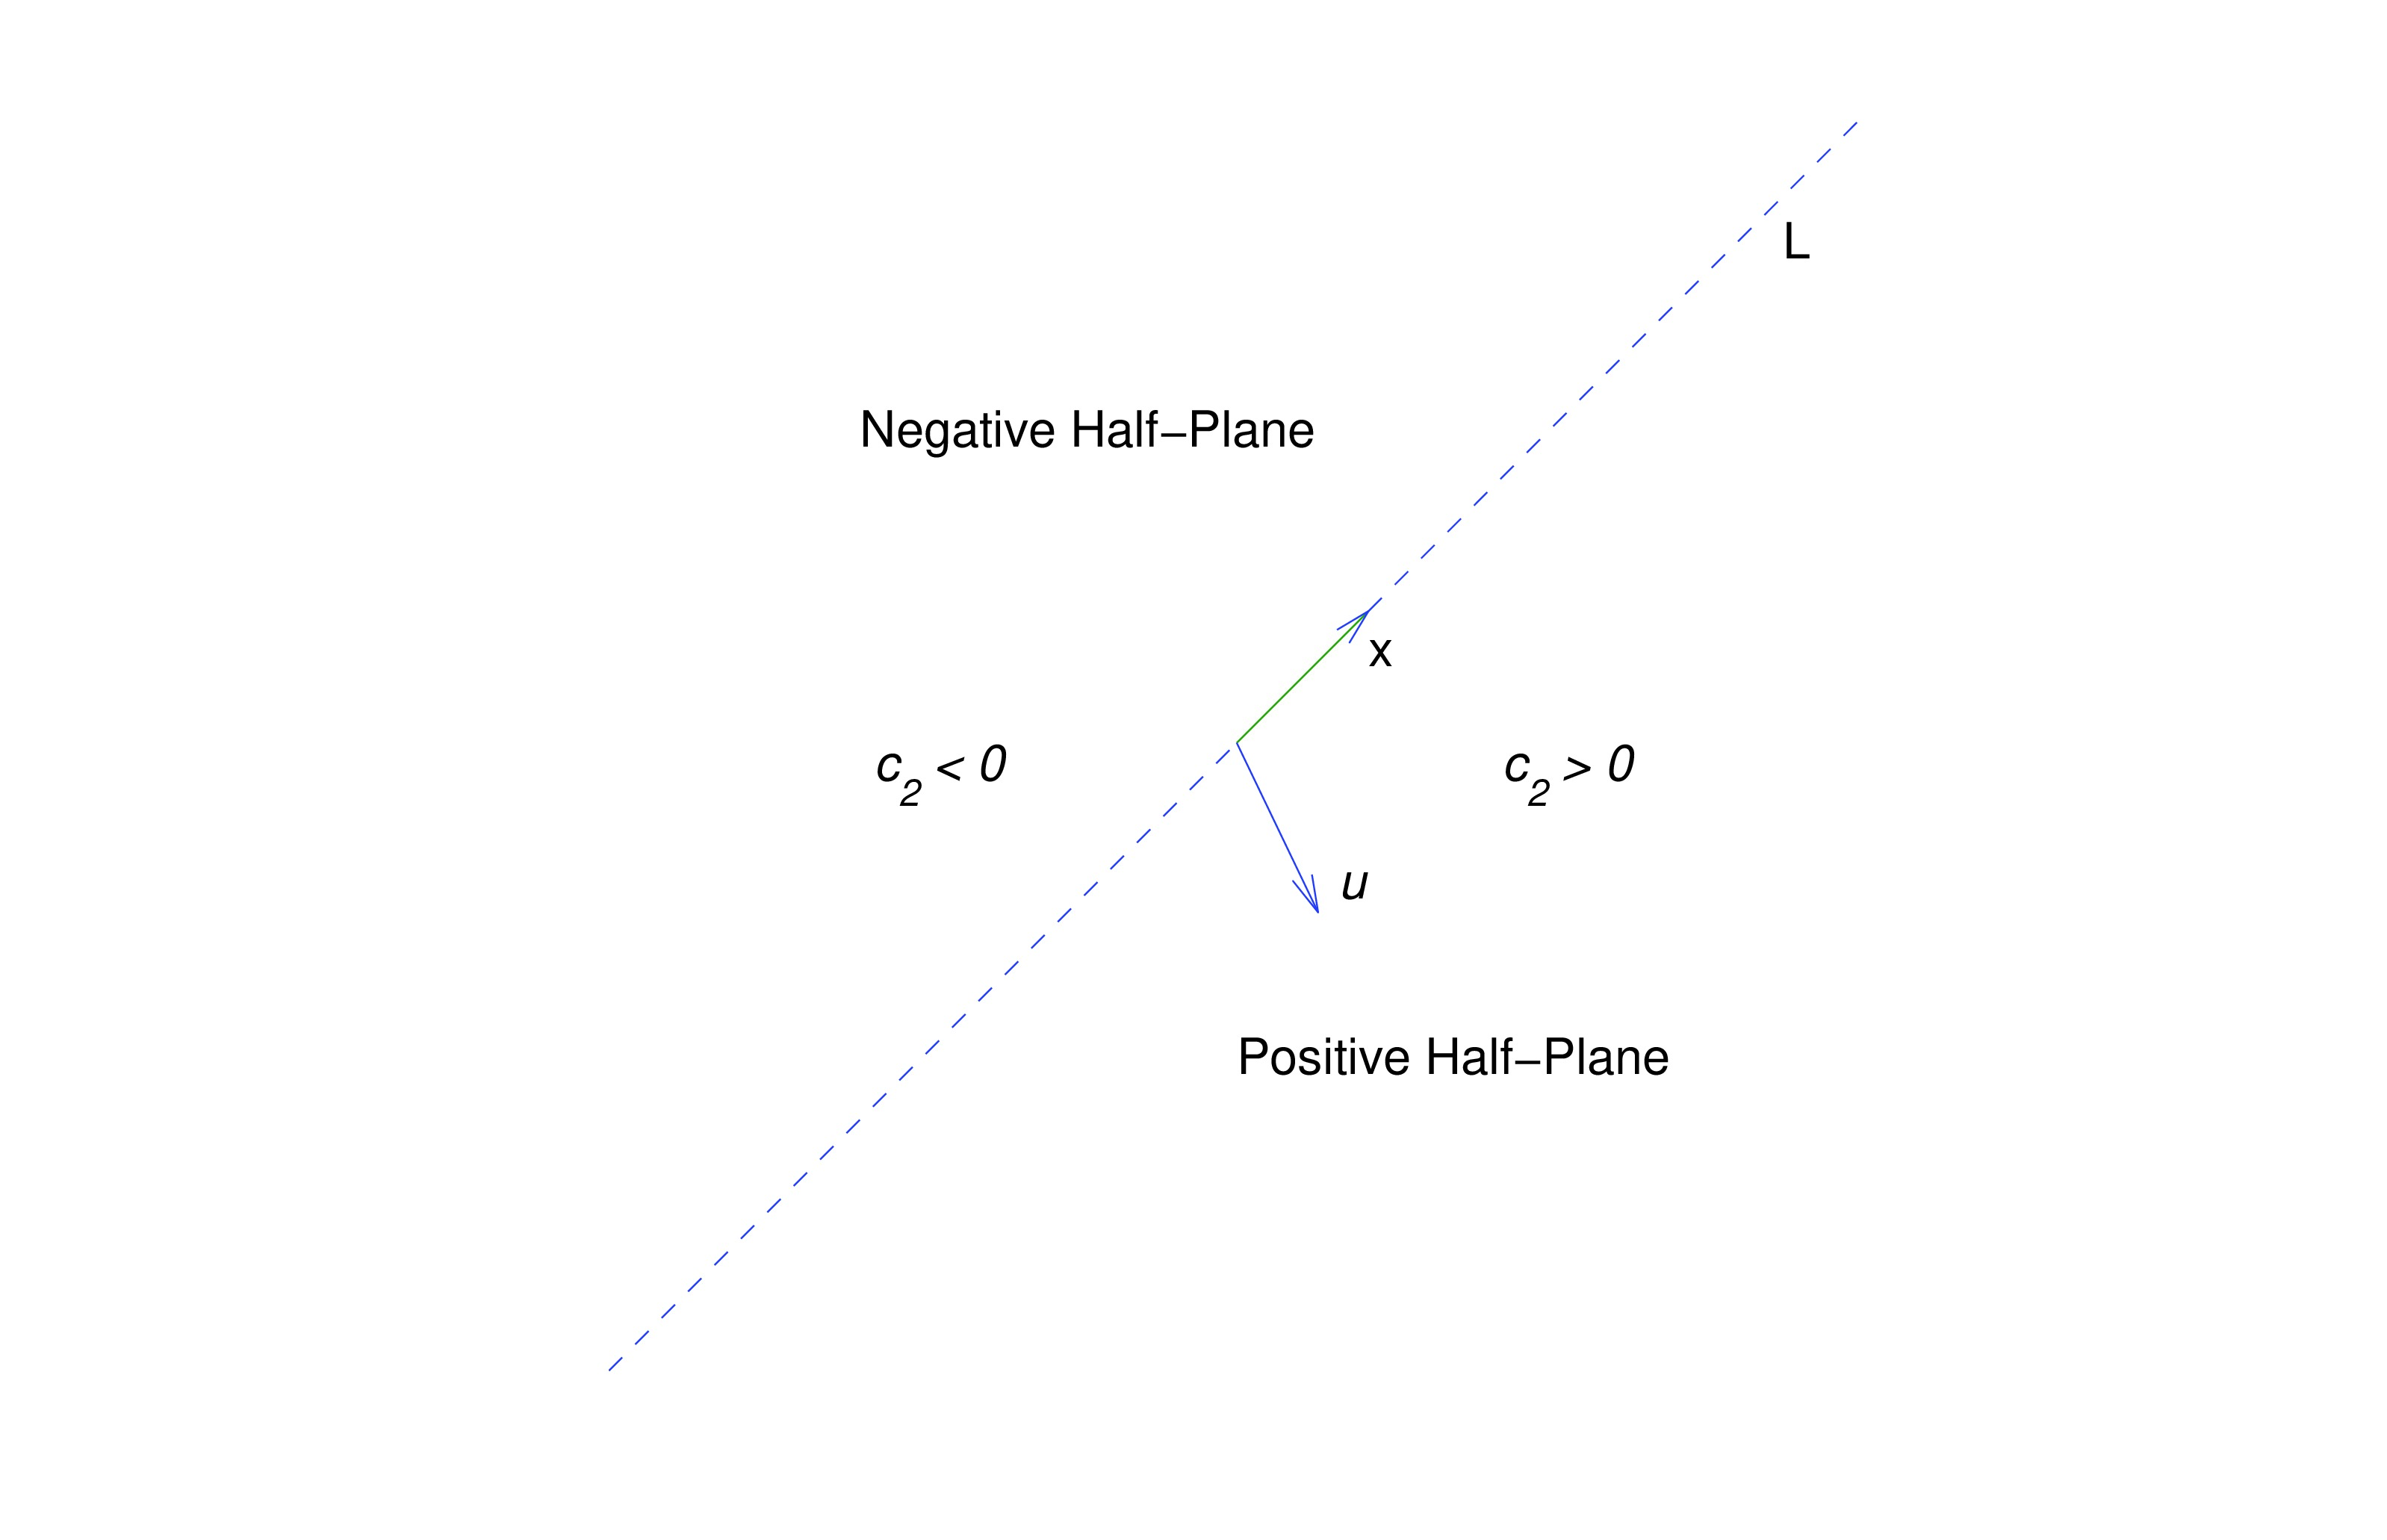
\includegraphics[height=1.5in]{fig100501.jpg} 
\end{image}


Let $L$ denote the line through the origin parallel to ${\bf x}$. By a
\dfn{half-line} of $L$ we mean either of the rays obtained by
removing the origin from $L$. Eqn.~\eqref{eq:10.5.20} is a parametric
equation of the half-line of $L$ in the direction of ${\bf x}$ if
$c_1>0$, or of the half-line of $L$ in the direction of $-{\bf x}$ if
$c_1<0$. The origin is the trajectory of the trivial solution ${\bf
y}\equiv{\bf 0}$.

Henceforth, we assume that $c_2\neq0$. In this case, the trajectory of
\eqref{eq:10.5.20} can't intersect $L$, since every point of $L$ is on a
trajectory obtained by setting $c_2=0$. Therefore the trajectory of
\eqref{eq:10.5.20} must lie entirely in one of the open half-planes
bounded
by $L$, but does not contain any point on $L$. Since the initial point
$(y_1(0),y_2(0))$ defined by ${\bf y}(0)=c_1{\bf x}_1+c_2{\bf u}$ is
on the trajectory, we can determine which half-plane contains the
trajectory from the sign of $c_2$, as shown in
the figure.
For convenience we'll call the half-plane where $c_2>0$ the
\dfn{positive half-plane}. Similarly, the-half plane where $c_2<0$ is
the \dfn{negative half-plane}. You should convince yourself %(Exercise~\ref{exer:10.5.35}) 
that even though there are infinitely
many vectors ${\bf u}$ that satisfy \eqref{eq:10.5.21}, they all define
the same positive and negative half-planes. In the figures simply
regard ${\bf u}$ as an arrow pointing to the positive half-plane,
since wen't attempted to give ${\bf u}$ its proper length or
direction in comparison with ${\bf x}$. For our purposes here, only the
relative orientation of ${\bf x}$ and ${\bf u}$ is important; that is,
whether the positive half-plane is to the right of an observer facing
the direction of ${\bf x}$, as in the figures below.

\begin{image}
 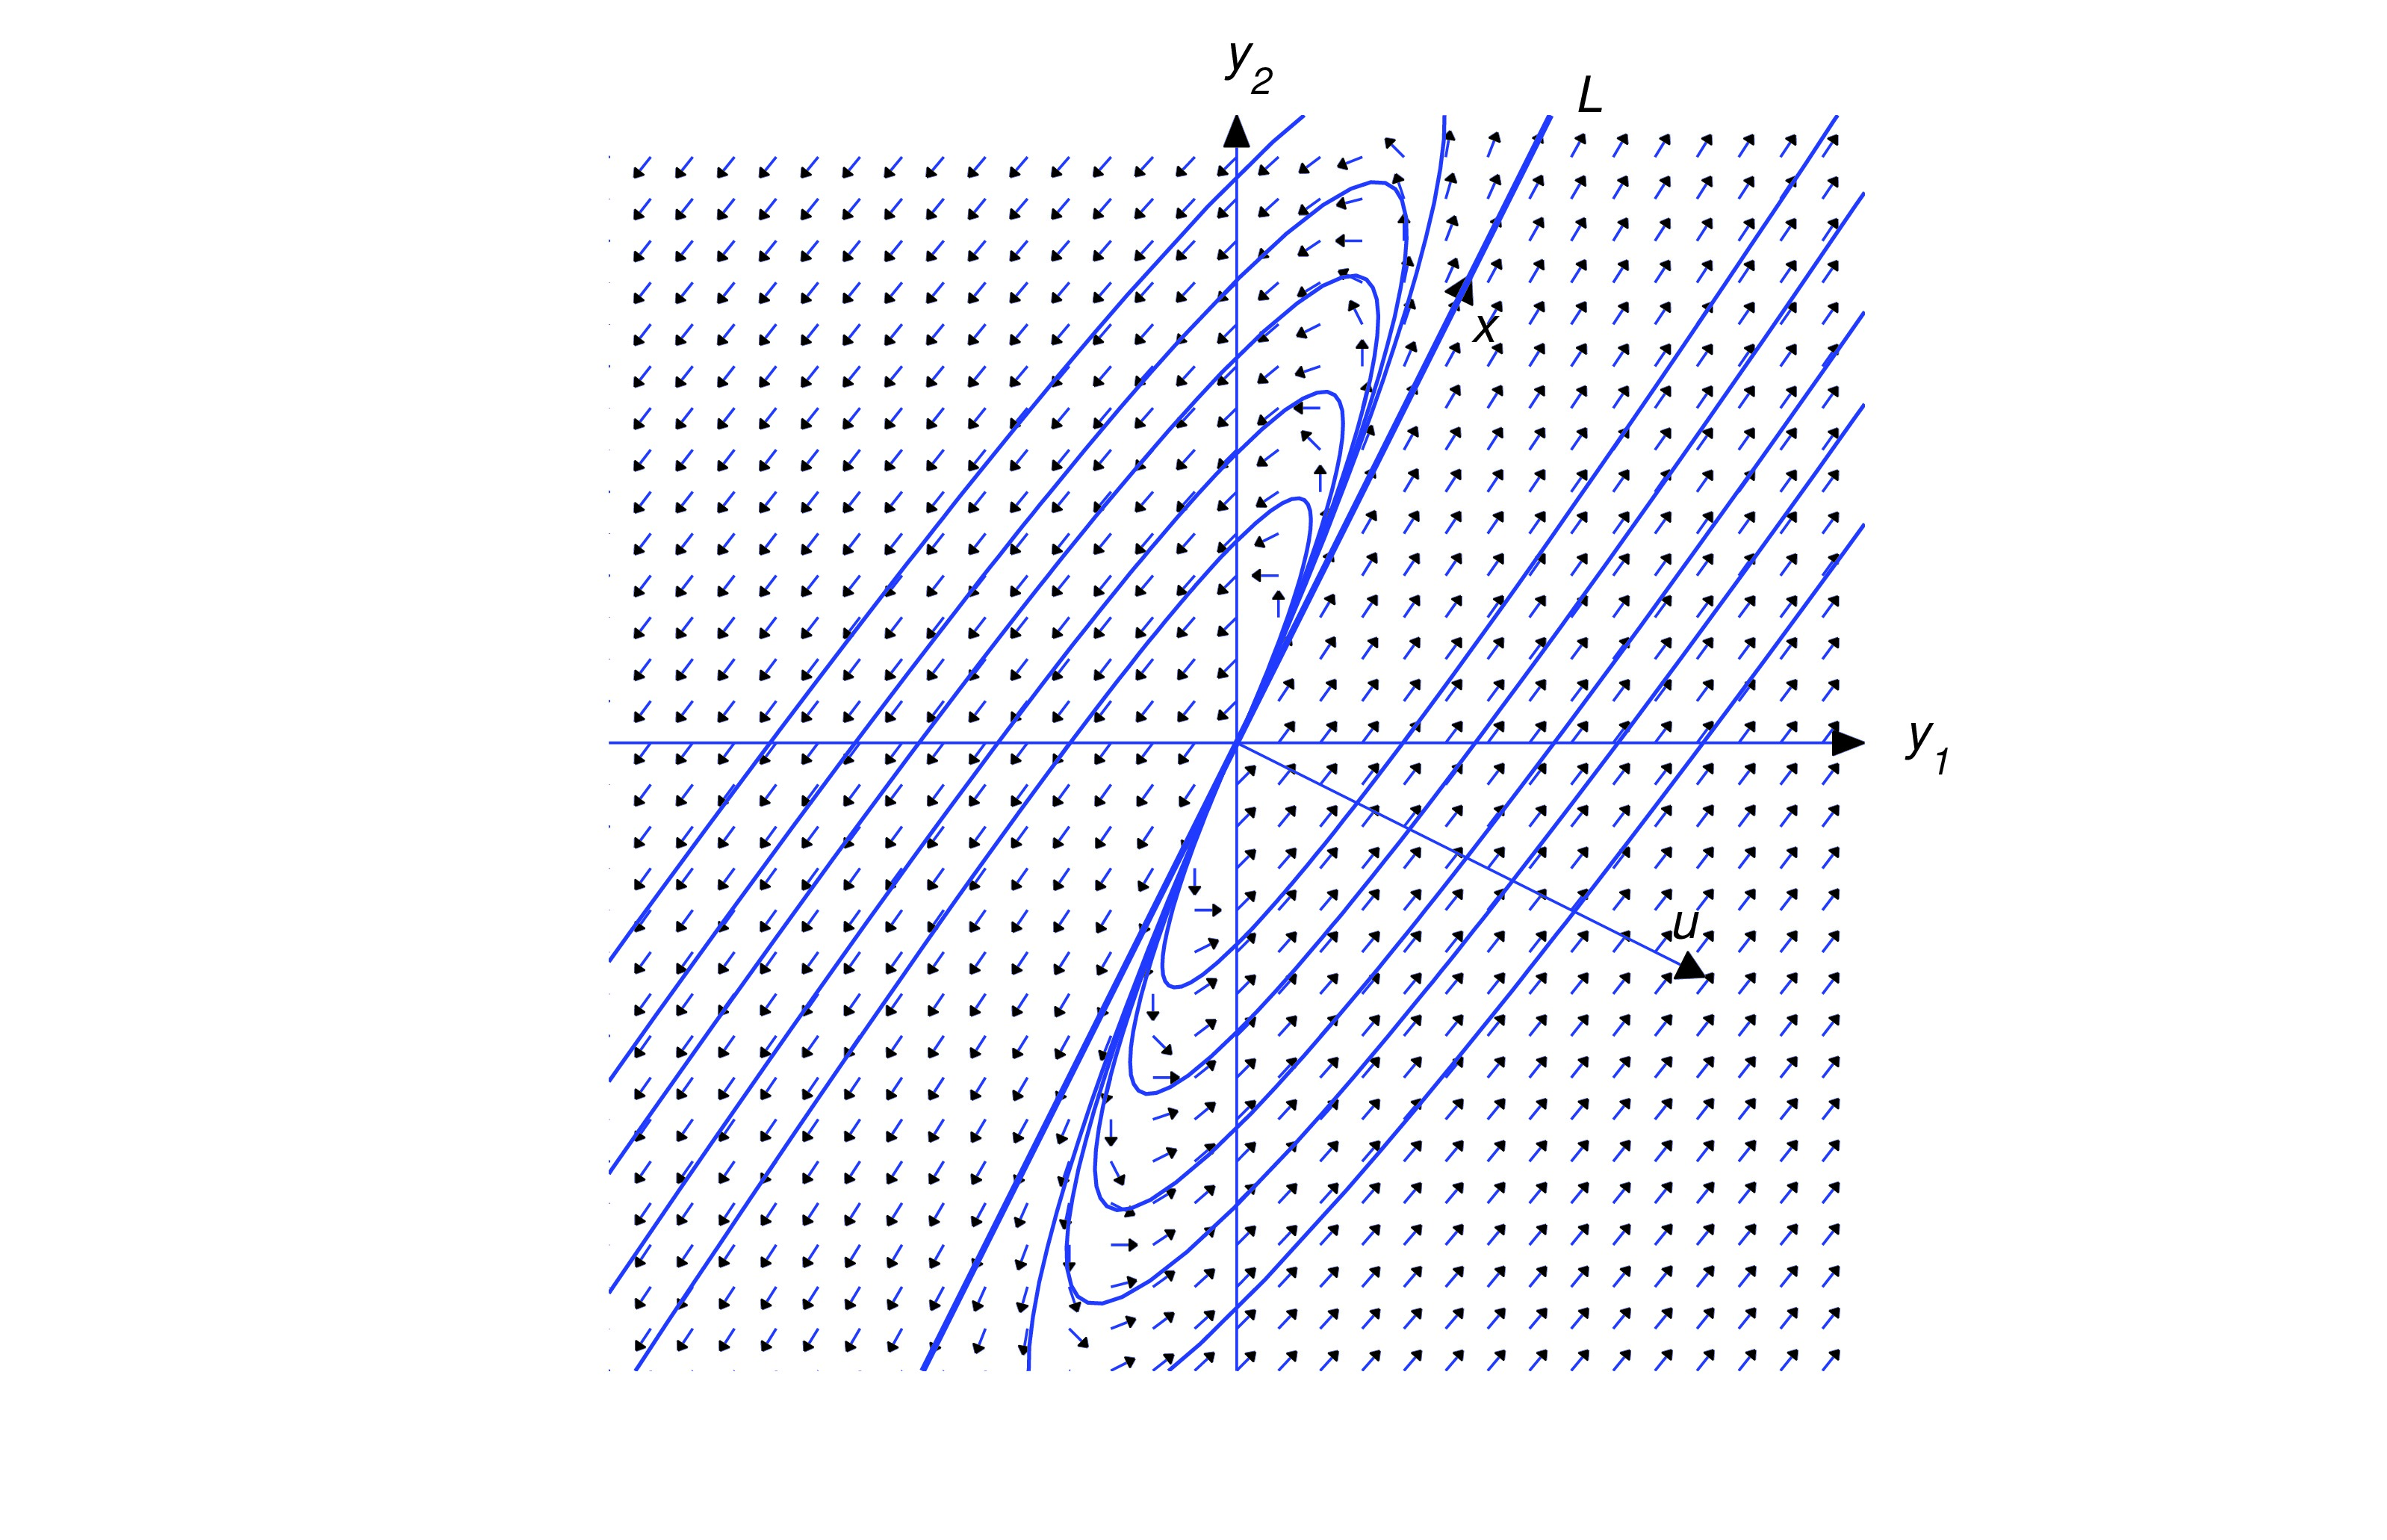
\includegraphics[height=1.5in]{fig100502.jpg} 
\end{image}

\begin{image}
 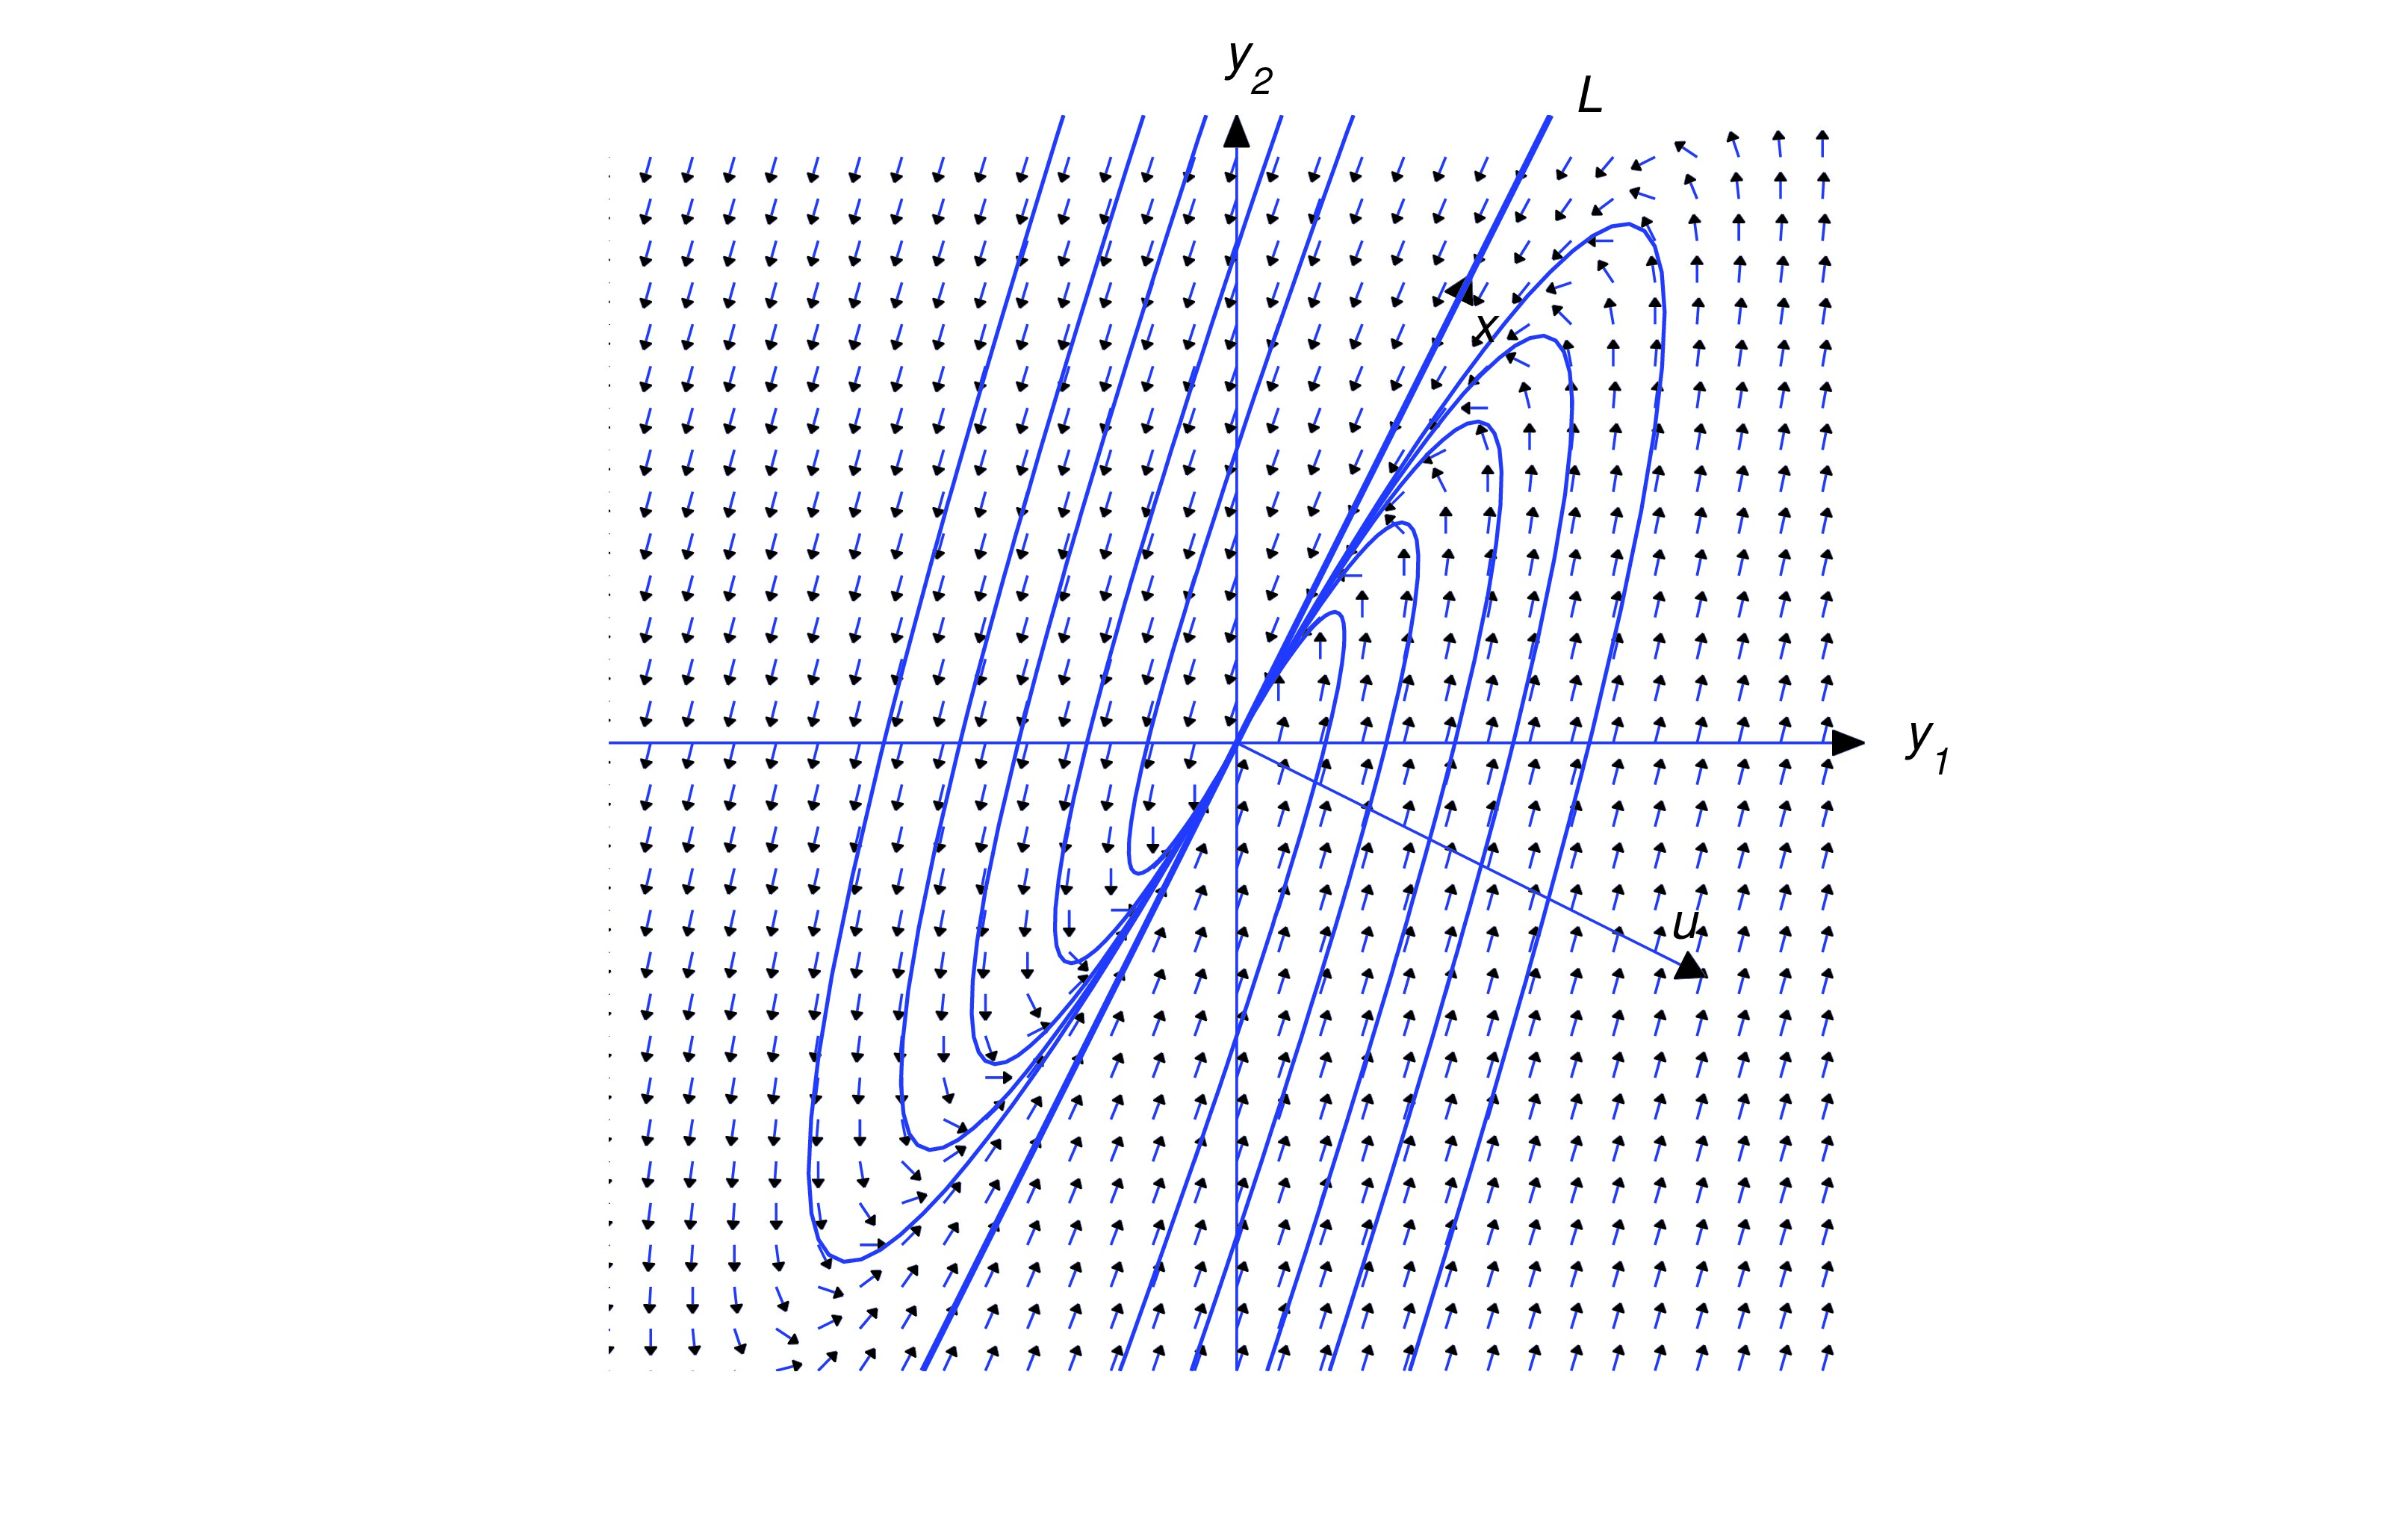
\includegraphics[height=1.5in]{fig100505.jpg} 
\end{image}



Or to the left of the observer, as shown below.

\begin{image}
 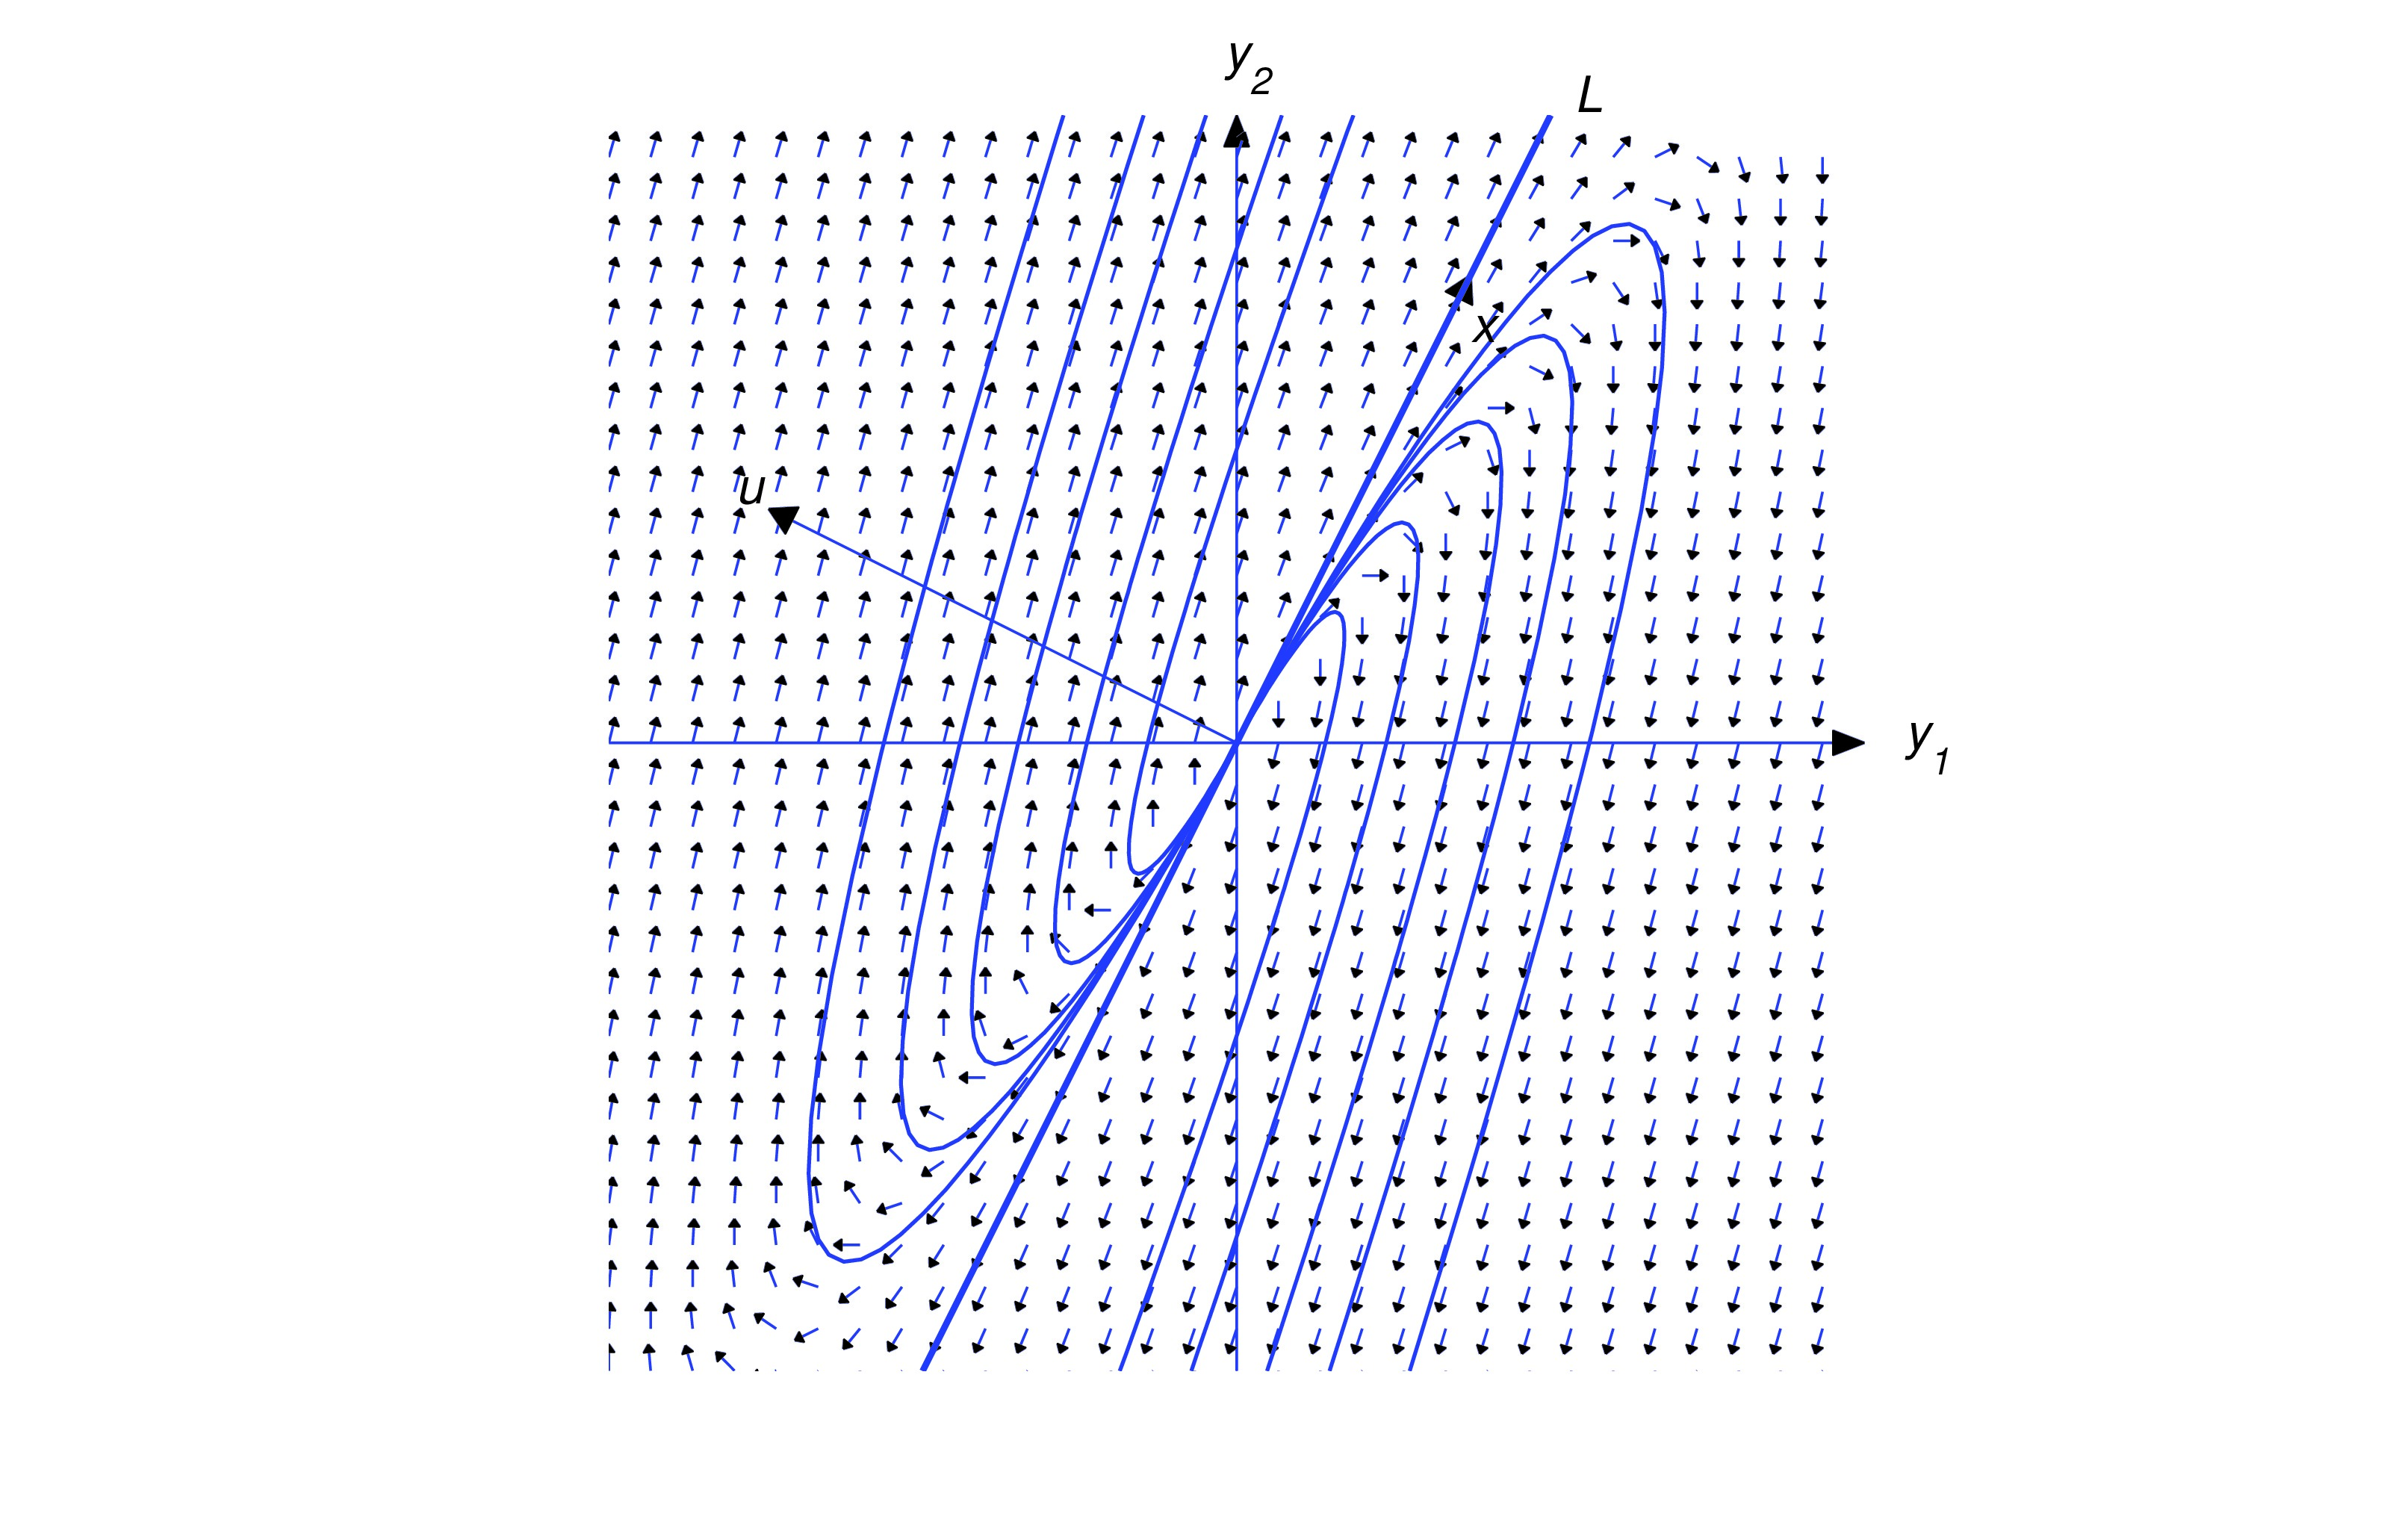
\includegraphics[height=1.5in]{fig100503.jpg} 
\end{image}

\begin{image}
 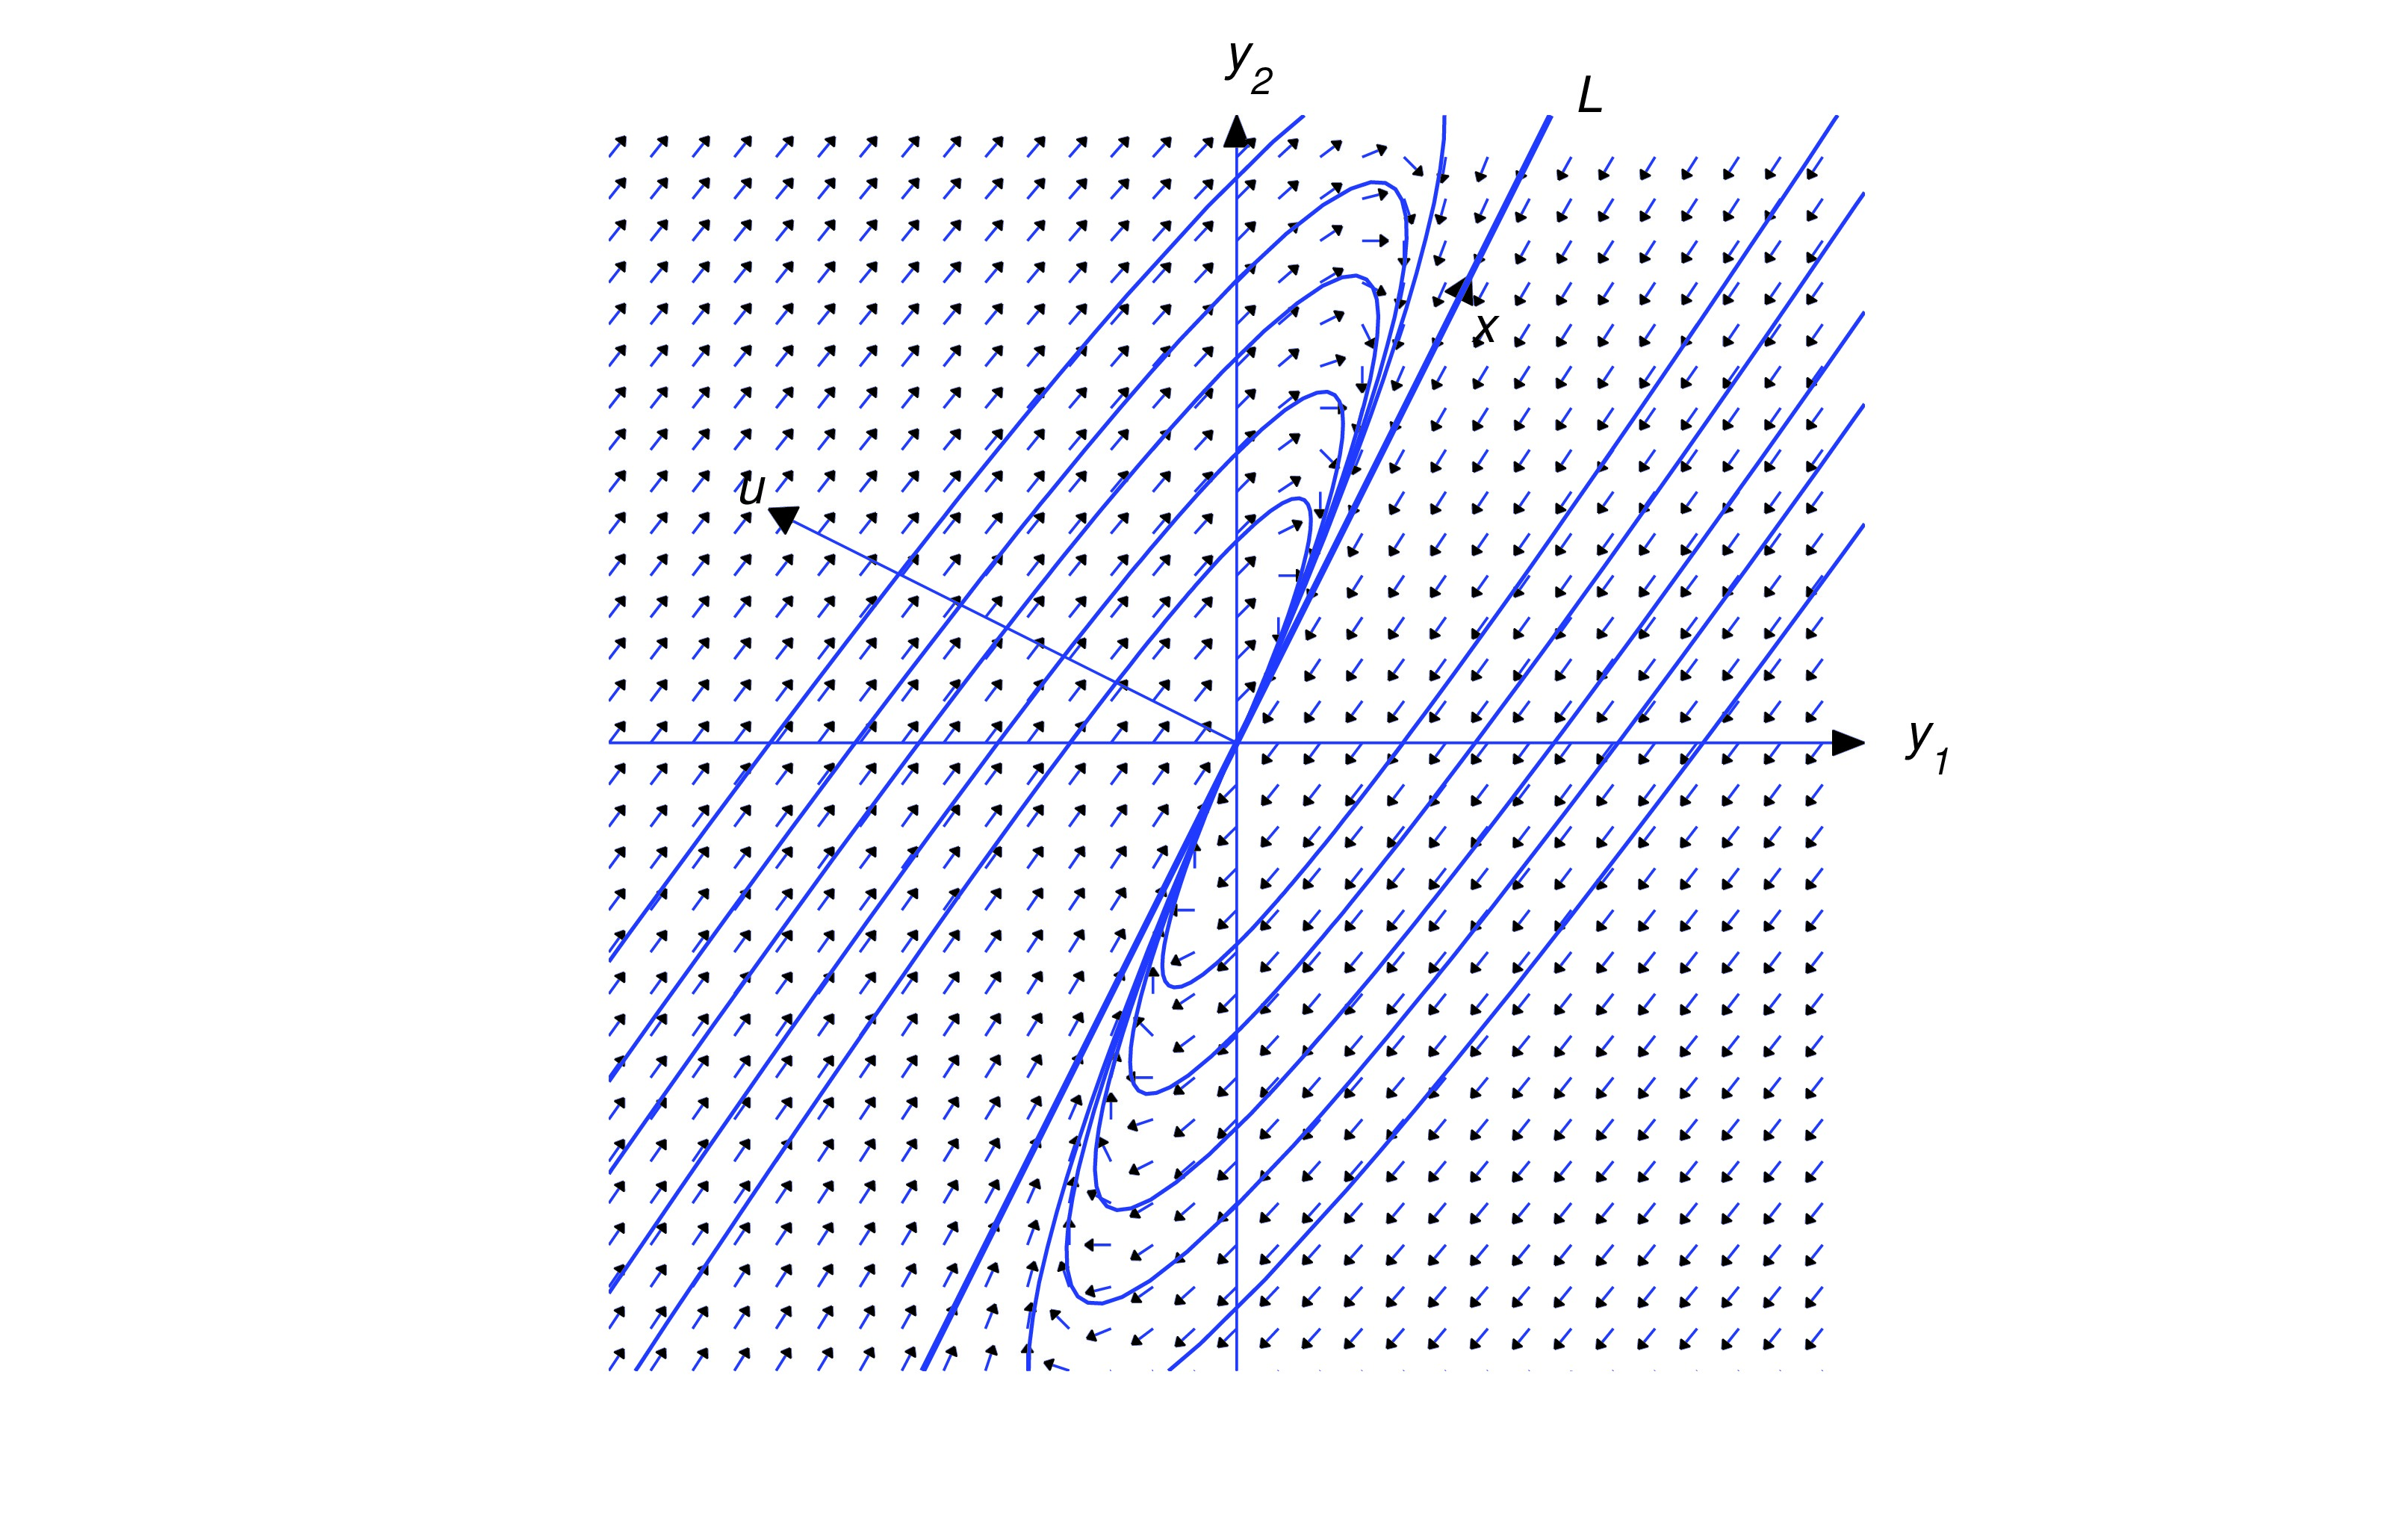
\includegraphics[height=1.5in]{fig100504.jpg} 
\end{image}

Multiplying \eqref{eq:10.5.20} by $e^{-\lambda_1t}$ yields
$$
e^{-\lambda_1t}{\bf y}(t)=c_1{\bf x}+c_2{\bf u}+c_2t
{\bf x}.
$$
Since the last term on the right is dominant when $|t|$ is large,
this provides the following information on the direction of ${\bf
y}(t)$:
\begin{enumerate}
\item % (a)
Along trajectories in the positive half-plane ($c_2>0$), the direction
of ${\bf y}(t)$ approaches the direction of ${\bf x}$ as $t\rightarrow\infty$
and the direction of $-{\bf x}$ as $t\rightarrow-\infty$.
\item % (b)
Along trajectories in the negative half-plane ($c_2<0$), the direction
of ${\bf y}(t)$ approaches the direction of $-{\bf x}$ as $t\rightarrow\infty$
and the direction of ${\bf x}$ as $t\rightarrow-\infty$.
\end{enumerate}

Since
$$
\lim_{t\rightarrow\infty}\|{\bf y}(t)\|=\infty\quad\mbox{and}\quad
\lim_{t\rightarrow-\infty}{\bf y}(t)={\bf 0}\quad\mbox{if}\quad\lambda_1>0,
$$
or
$$
\lim_{t-\rightarrow\infty}\|{\bf y}(t)\|=\infty\quad\mbox{and}\quad
\lim_{t\rightarrow\infty}{\bf y}(t)={\bf 0}\quad\mbox{if}\quad\lambda_1<0,
$$
 there are four possible patterns for the trajectories
of \eqref{eq:10.5.19}, depending upon the signs of $c_2$ and $\lambda_1$.

\begin{image}
 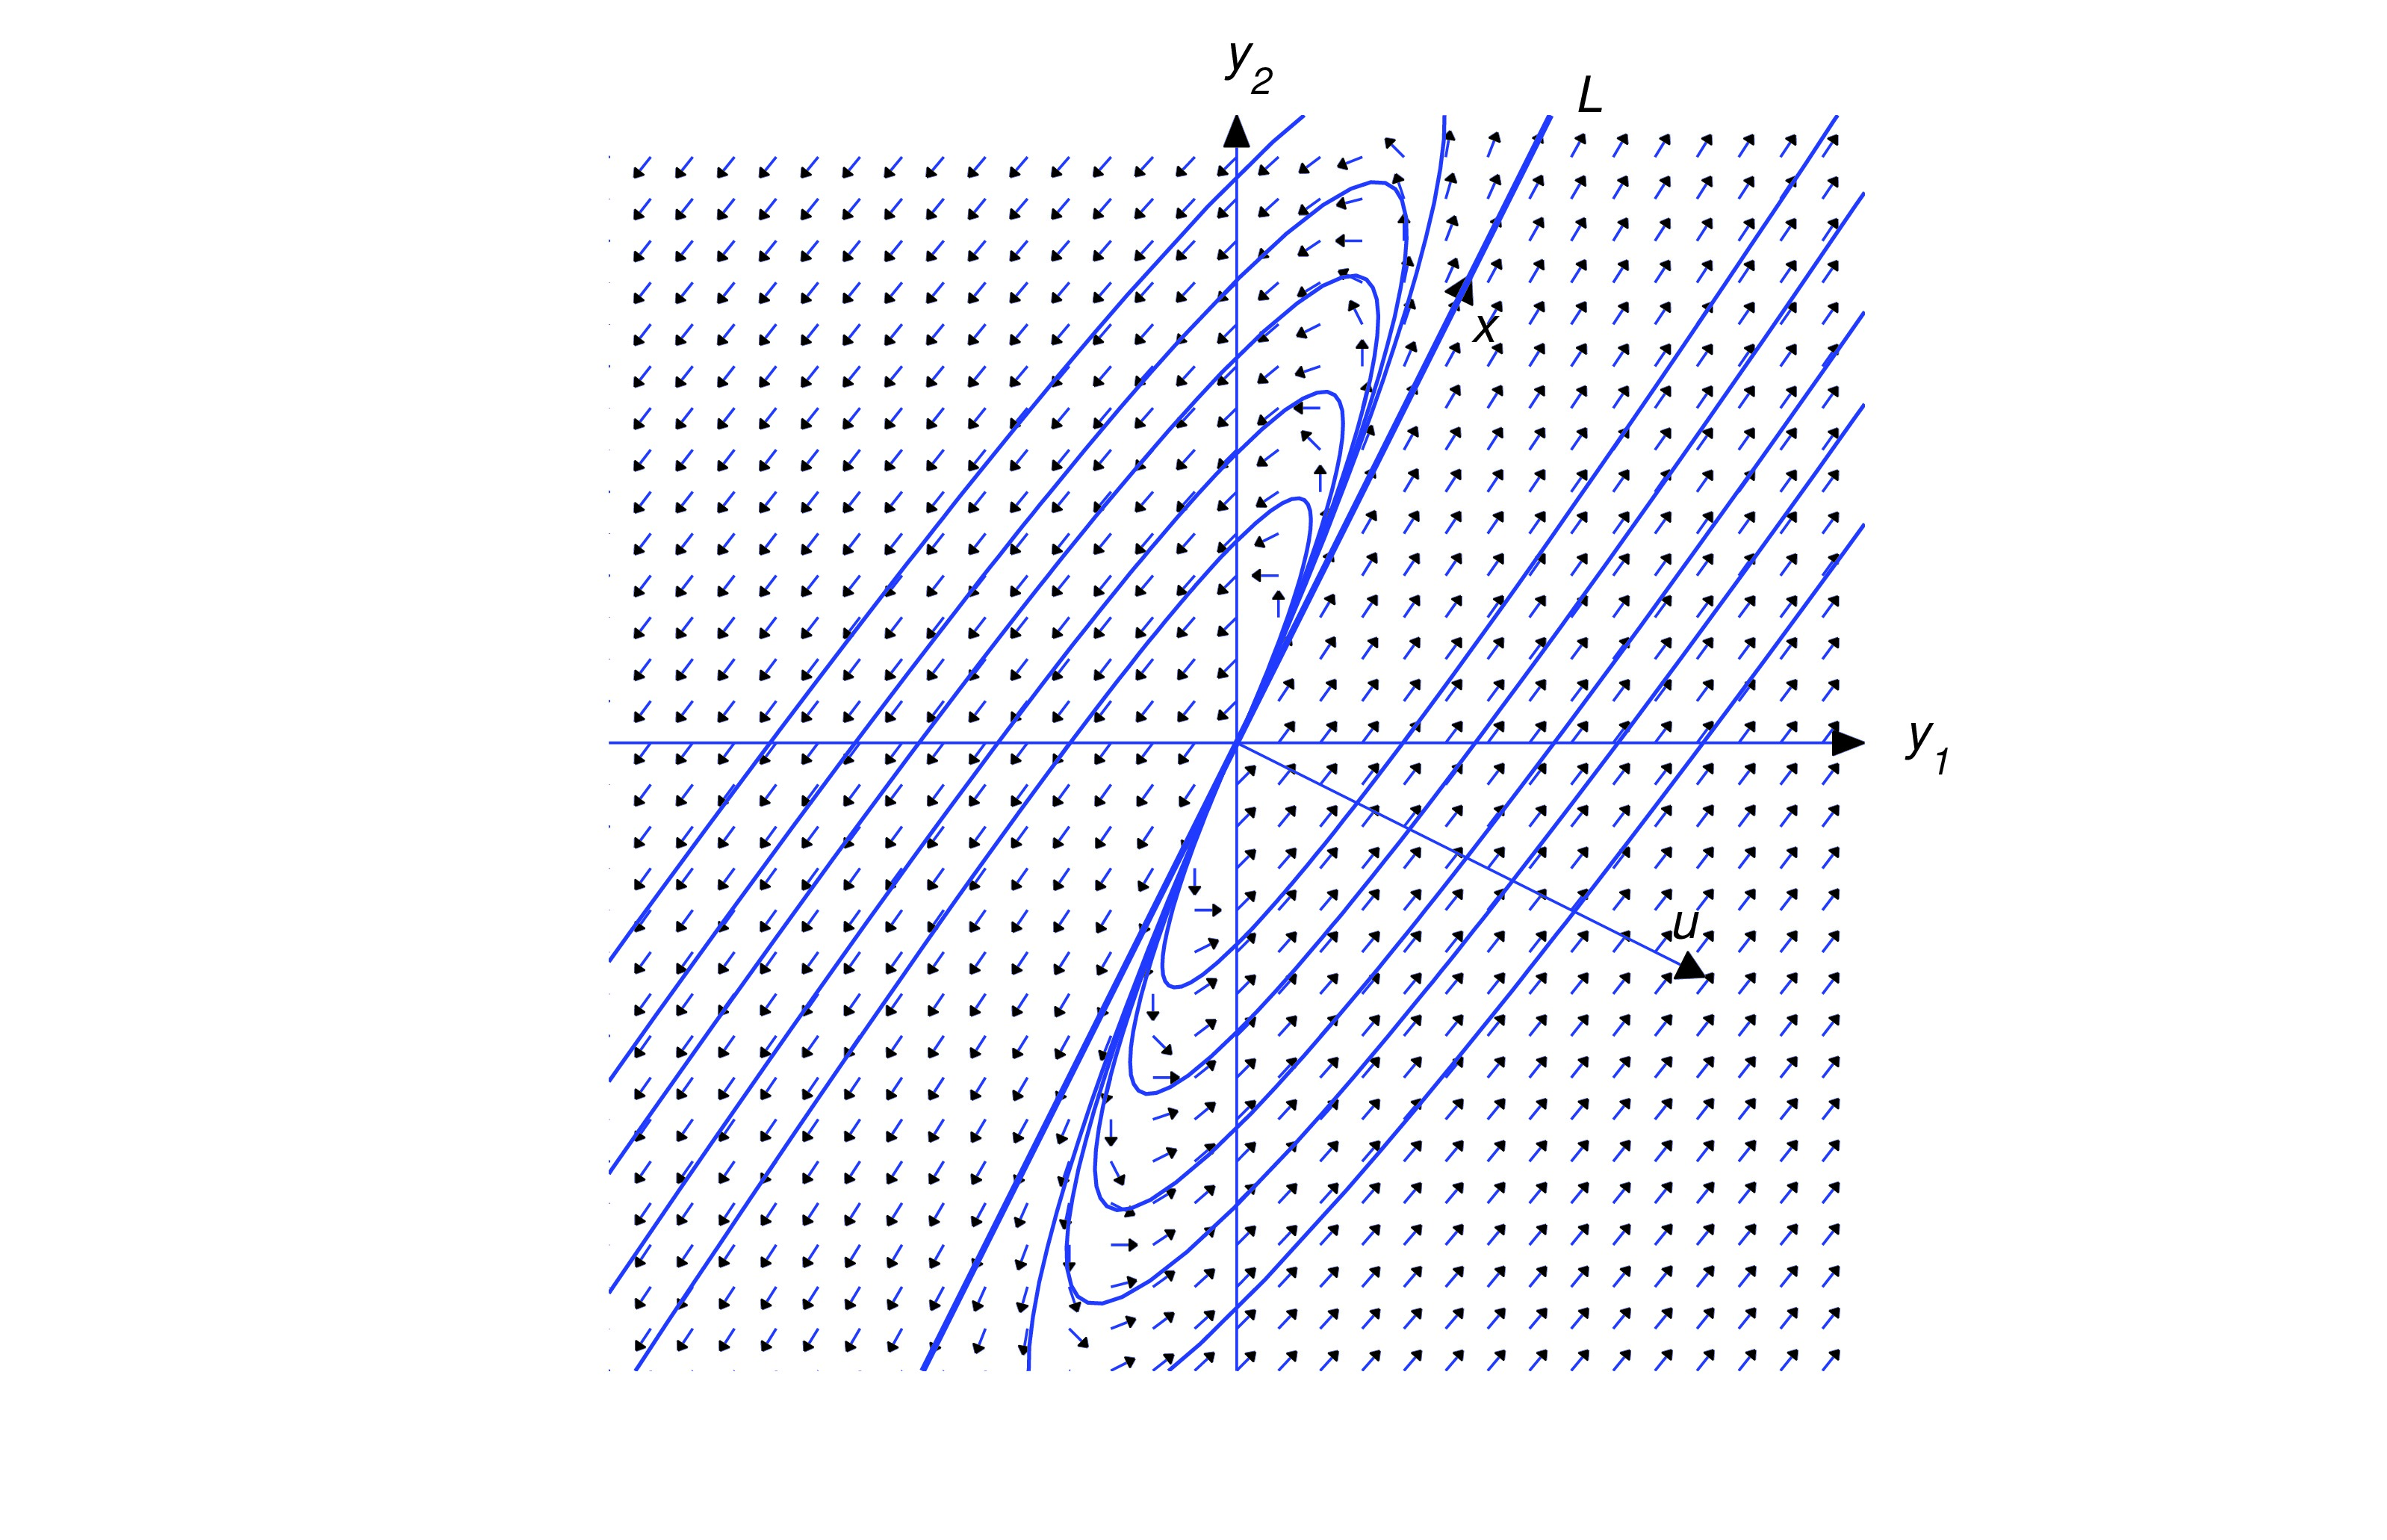
\includegraphics[height=1.5in]{fig100502.jpg} 
\end{image}

\begin{image}
 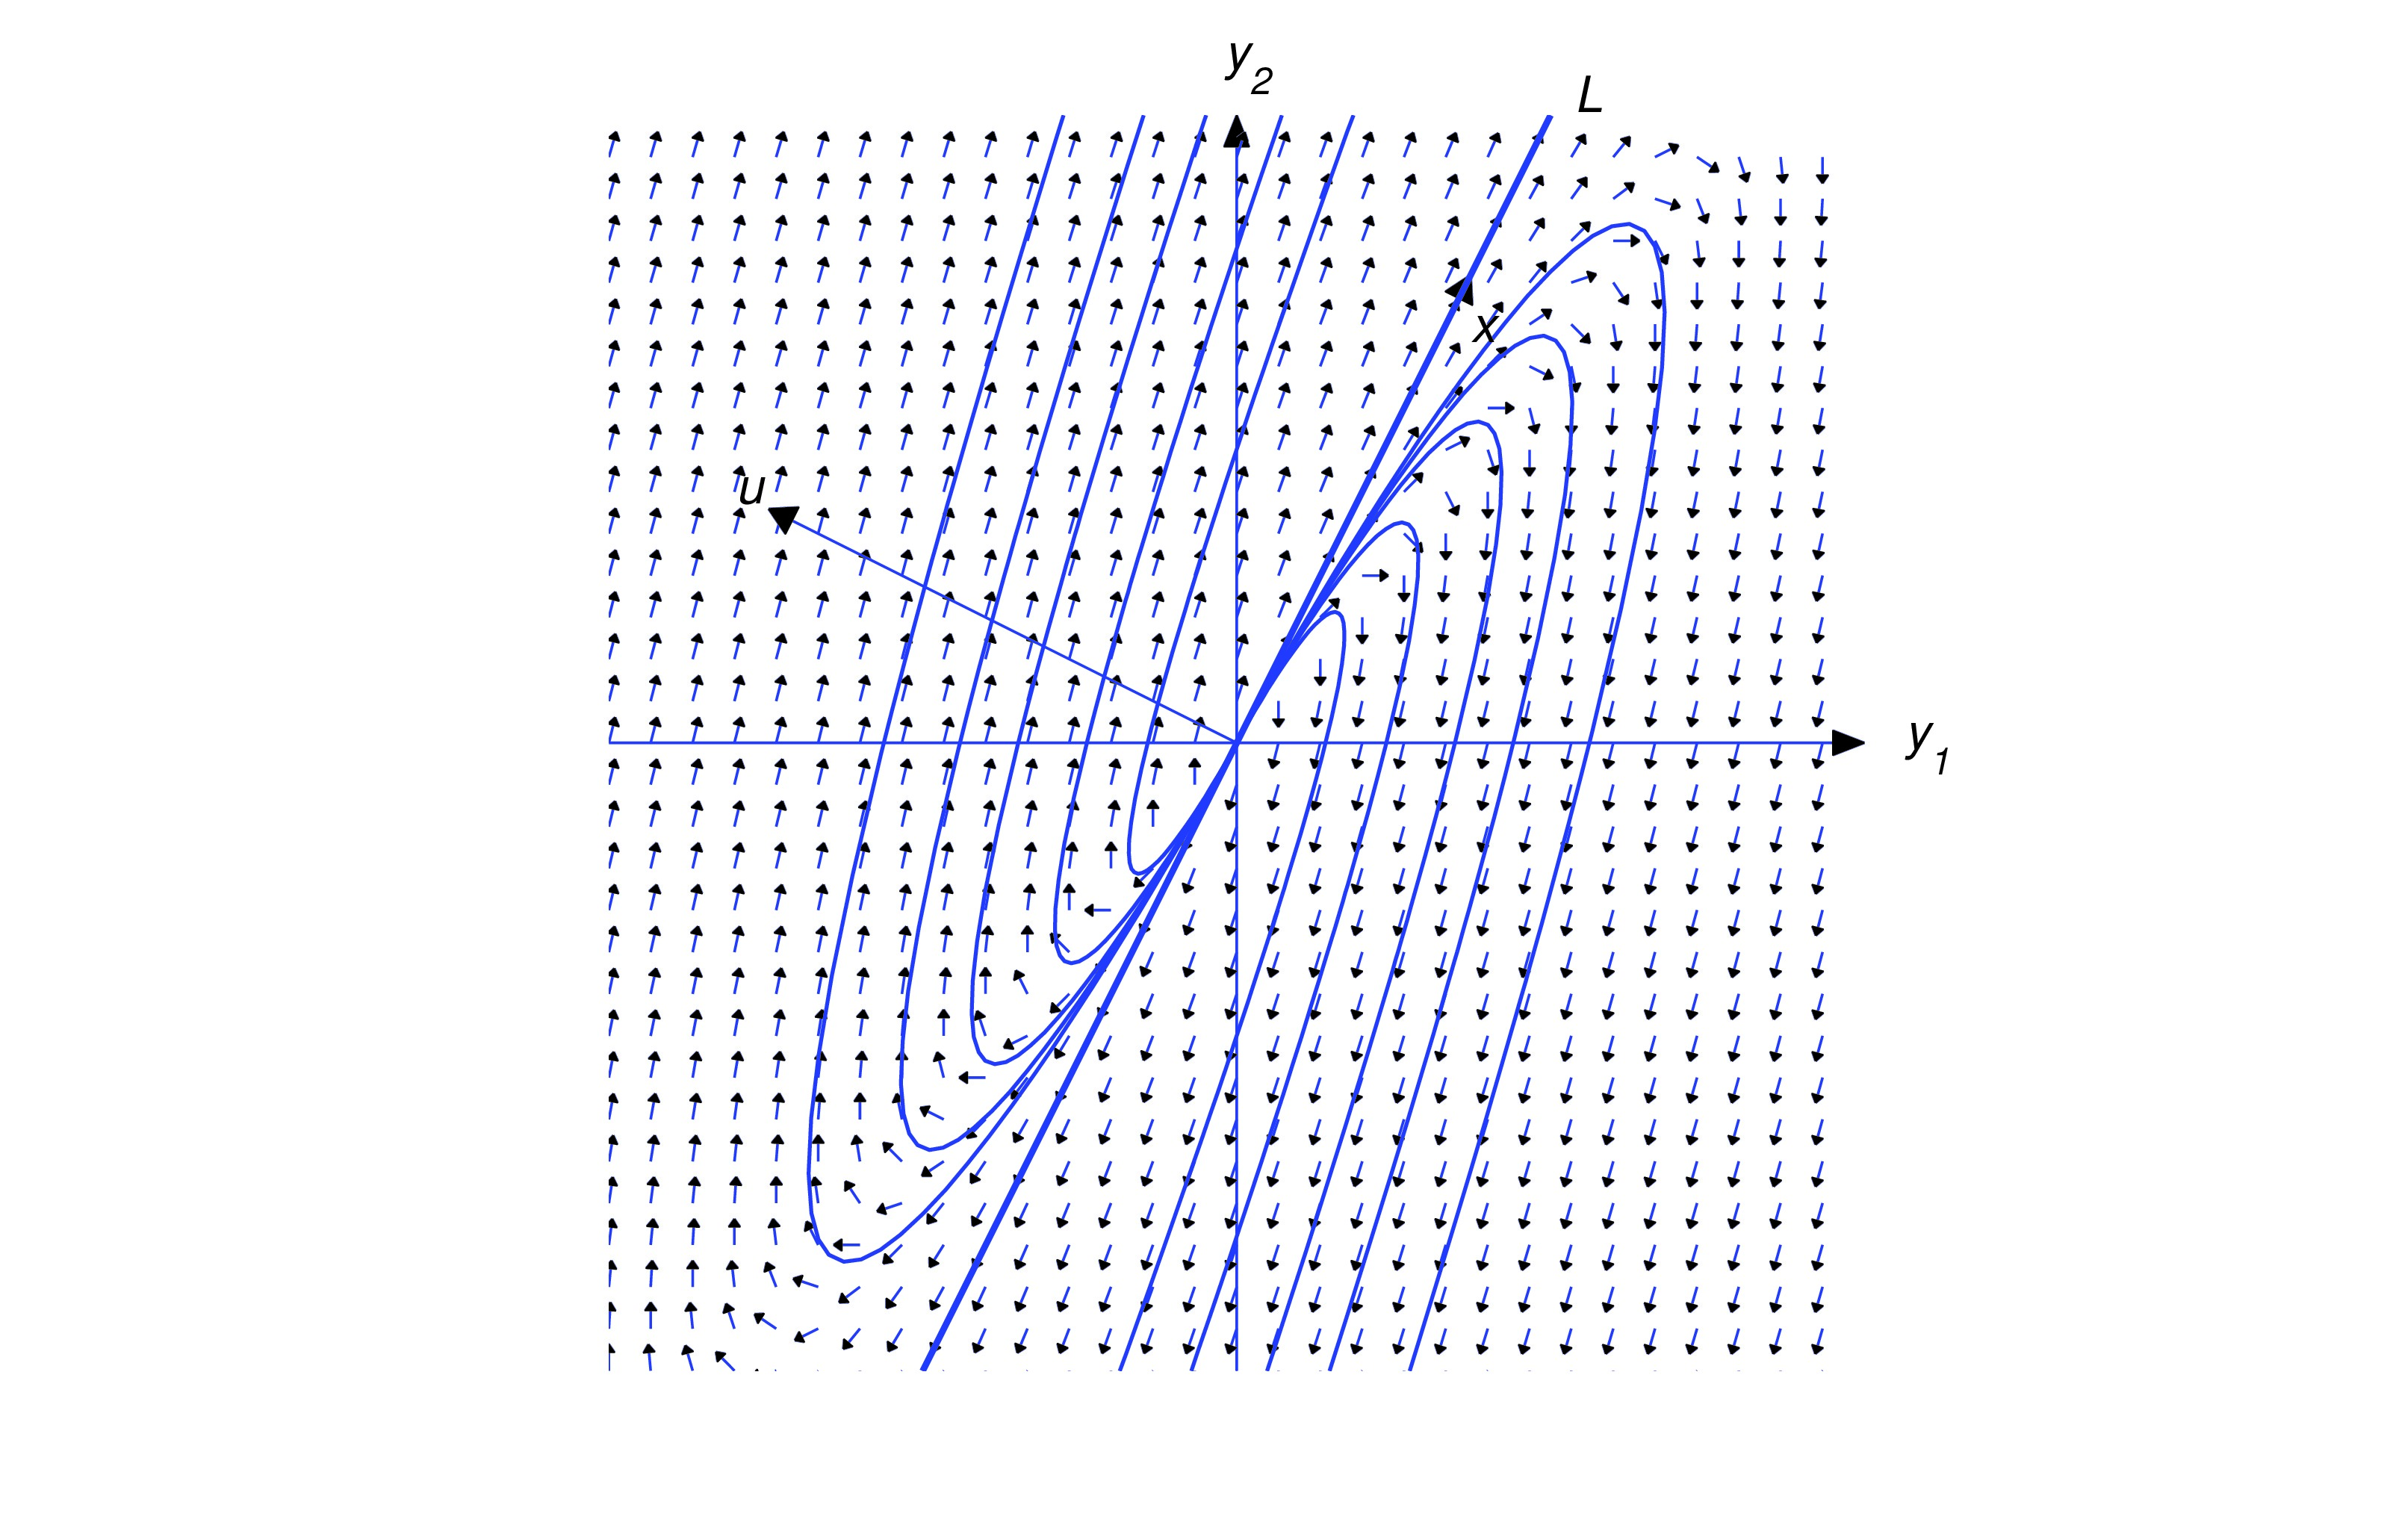
\includegraphics[height=1.5in]{fig100503.jpg} 
\end{image}

\begin{image}
 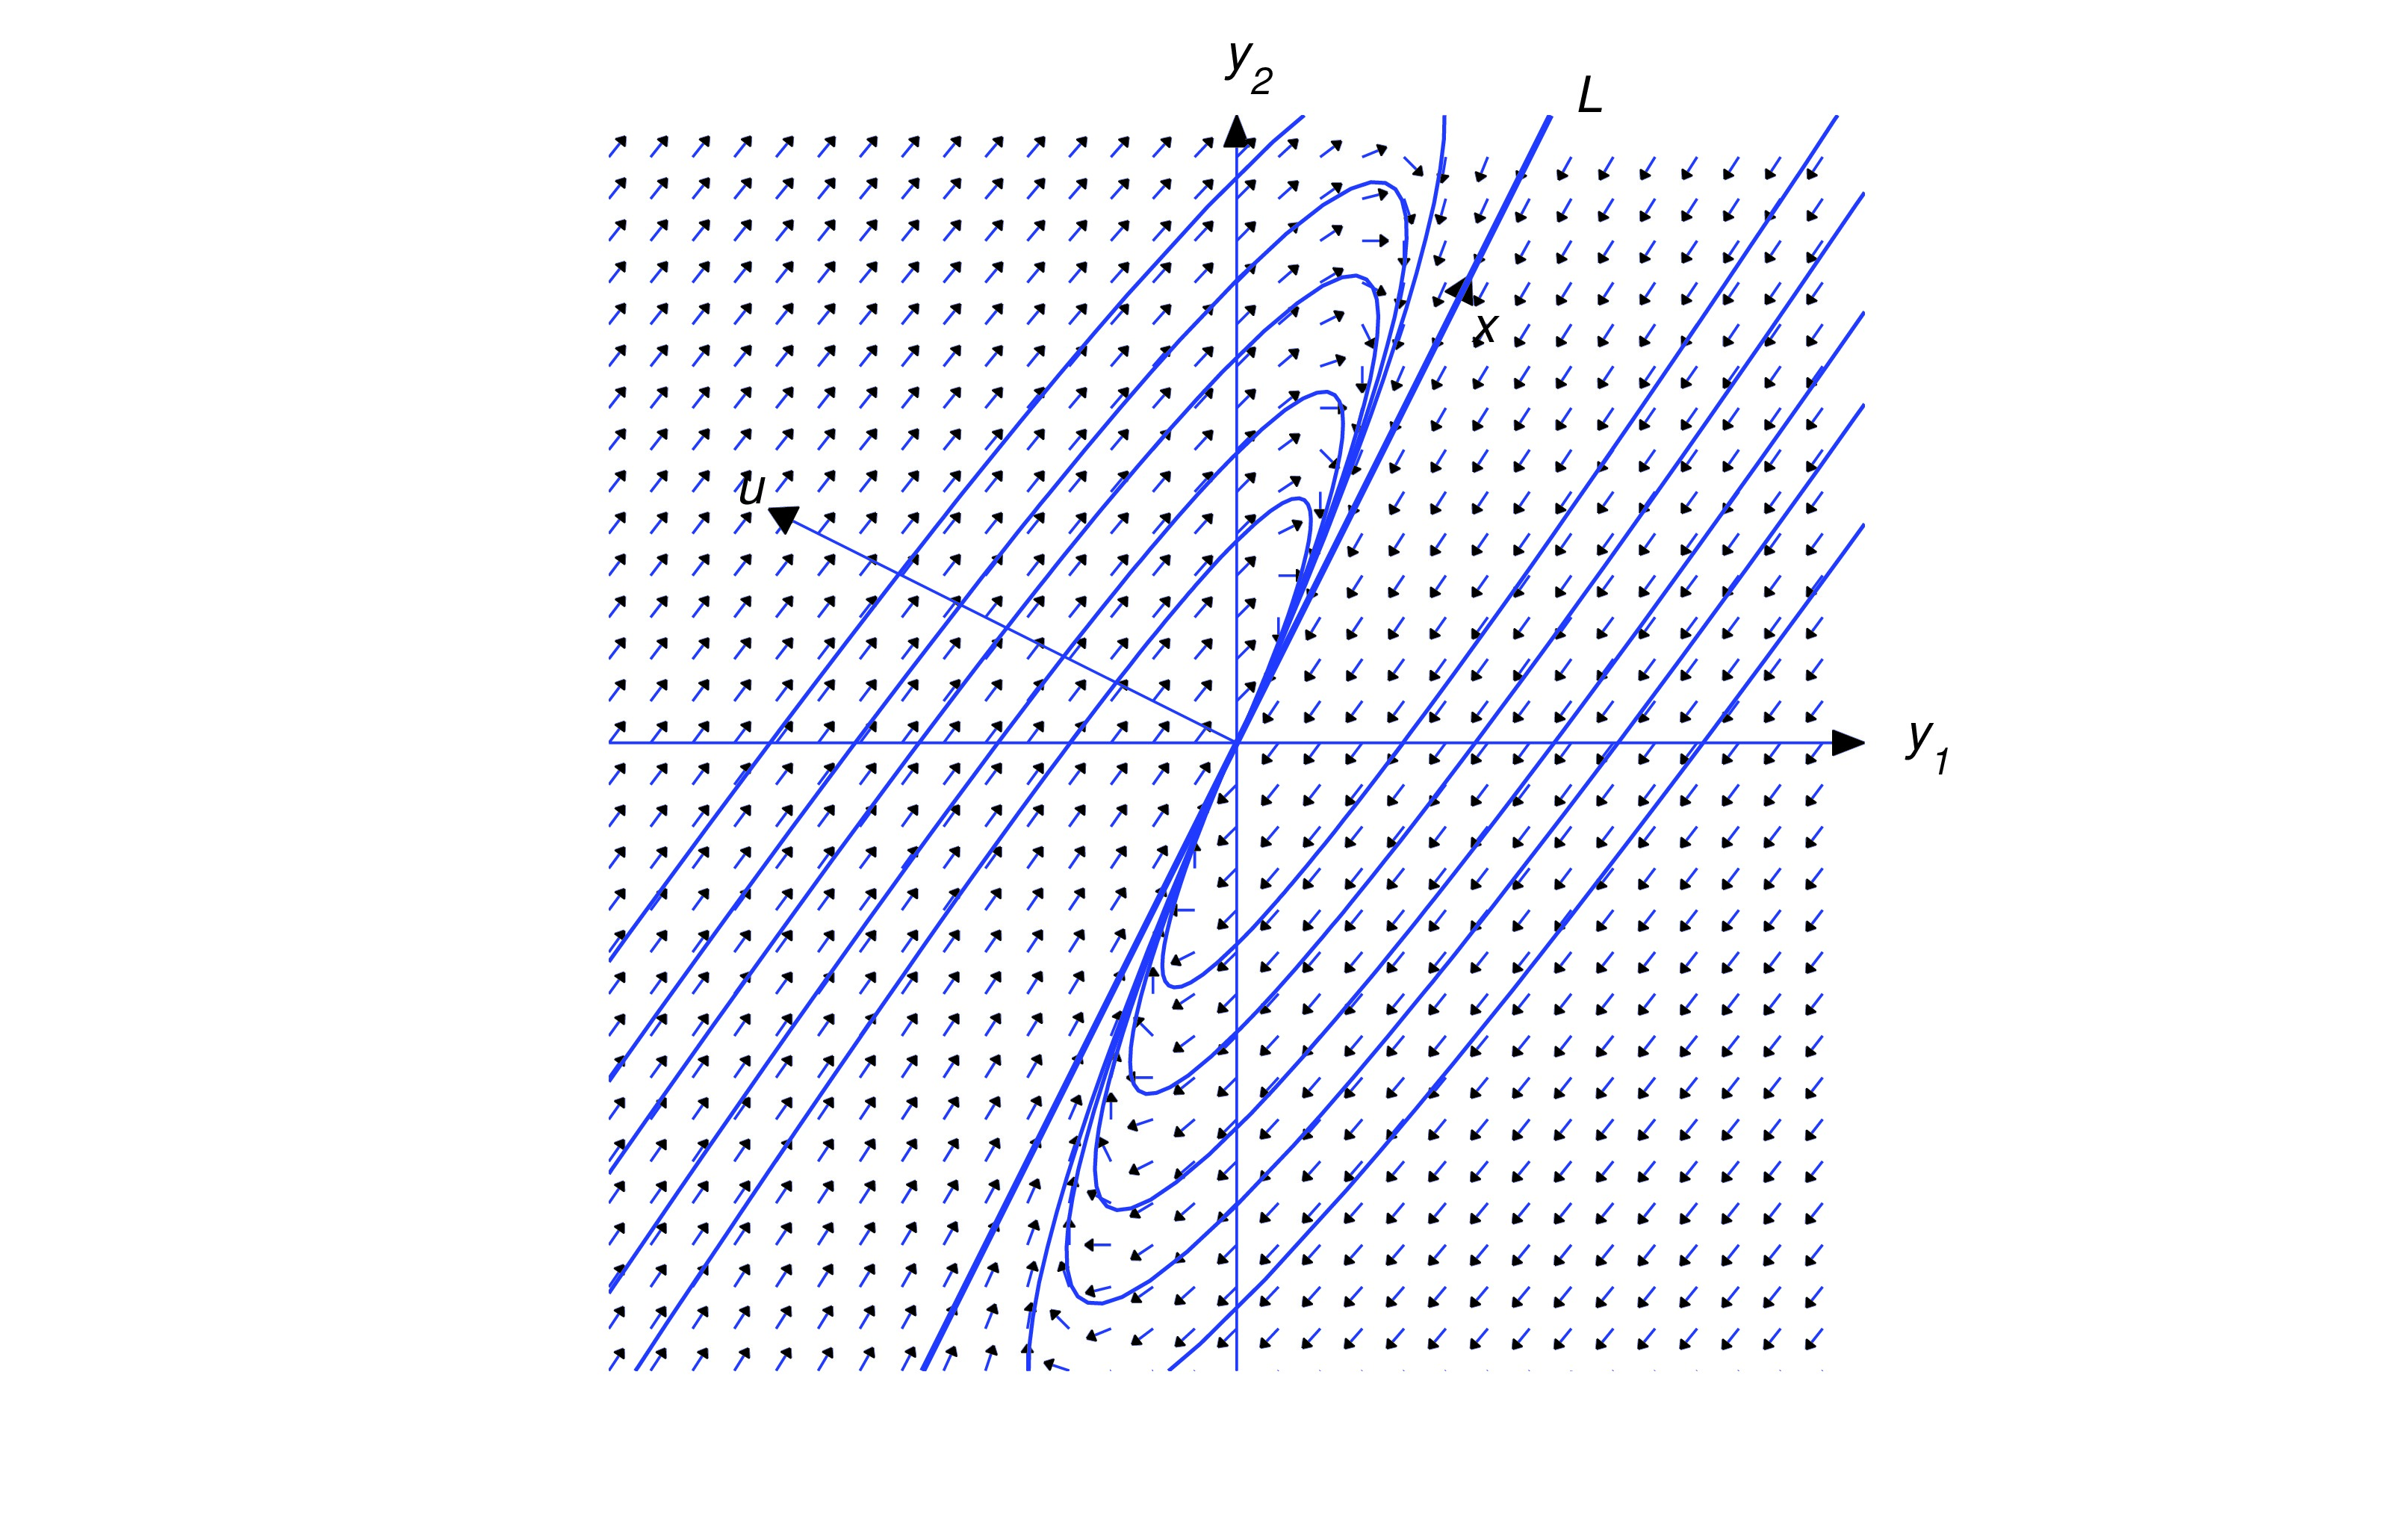
\includegraphics[height=1.5in]{fig100504.jpg} 
\end{image}

\begin{image}
 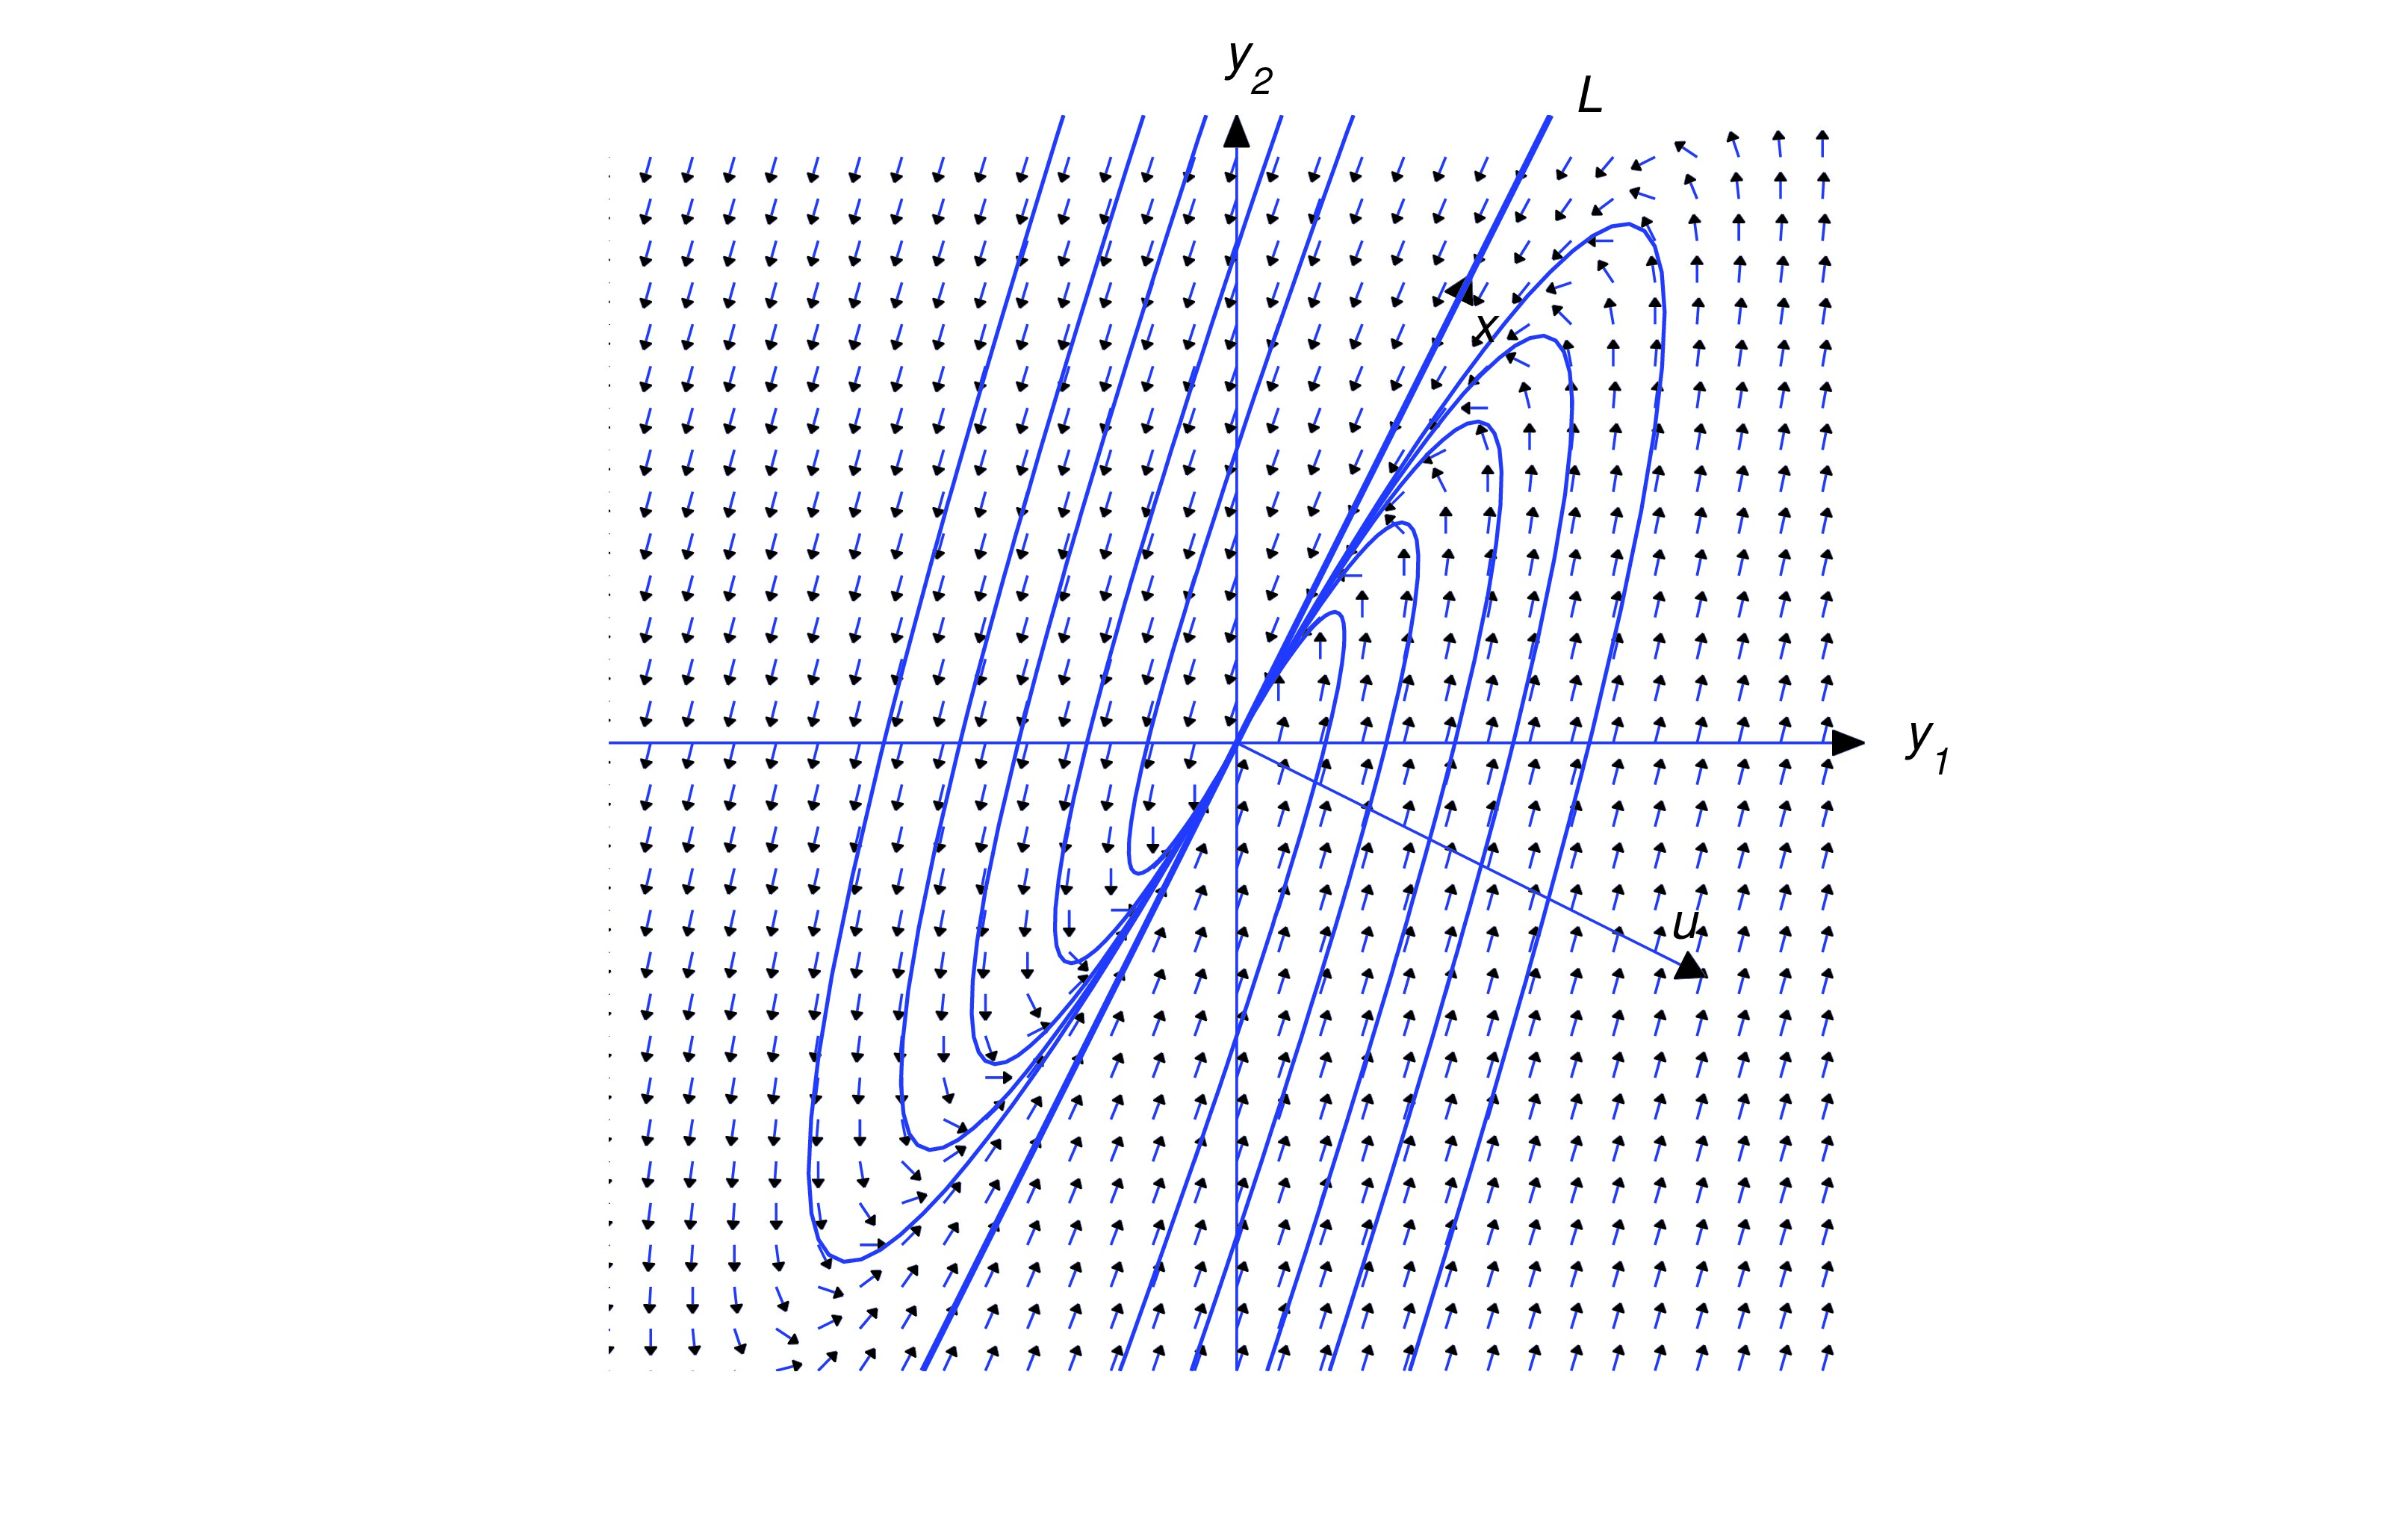
\includegraphics[height=1.5in]{fig100505.jpg} 
\end{image}

The above figures illustrate these patterns, and
reveal the following principle:
\begin{observation}
If $\lambda_1$ and $c_2$ have the same sign then the
direction of
the trajectory approaches the direction of $-{\bf x}$ as $\norm{{\bf y}}\rightarrow 0$ and the direction of ${\bf x}$ as $\norm{{\bf y}}\rightarrow\infty$. If
$\lambda_1$ and $c_2$ have opposite signs then the direction of the
trajectory approaches the direction of ${\bf x}$ as $\norm{{\bf y}}\rightarrow0$
and the direction of $-{\bf x}$ as $\norm{{\bf y}}\rightarrow\infty$.
\end{observation}




\section*{Text Source}
Trench, William F., "Elementary Differential Equations" (2013). Faculty Authored and Edited Books \& CDs. 8. (CC-BY-NC-SA)

\href{https://digitalcommons.trinity.edu/mono/8/}{https://digitalcommons.trinity.edu/mono/8/}


\end{document}